\documentclass[a4paper,preprint,12pt,numbers]{elsarticle}
\usepackage[T1]{fontenc}
\usepackage[a4paper,margin=1in]{geometry}
\usepackage{newtxtext,newtxmath}
\usepackage{amsmath,amssymb,amsfonts,mathrsfs}
\usepackage{graphicx}
\usepackage{booktabs,multirow,threeparttable}
\usepackage{longtable,array}
\usepackage{bm,mathtools}
\usepackage{enumitem}
\usepackage{xcolor}
\usepackage{textcomp}
\usepackage{microtype}
\usepackage{url}
\usepackage{hyperref}
\hypersetup{hidelinks}
\emergencystretch=2em
\newcommand{\bmx}{\bm{x}}
\newcommand{\bmk}{\bm{k}}
\newcommand{\bmu}{\bm{u}}
\newcommand{\bmv}{\bm{v}}
\newcommand{\bmK}{\bm{K}}
\newcommand{\bmM}{\bm{M}}
\newcommand{\bmB}{\bm{B}}
\newcommand{\bmR}{\bm{R}}
\newcommand{\bmT}{\bm{T}}
\newcommand{\bmC}{\bm{C}}
\newcommand{\barw}{\bar{\omega}}
\newcommand{\bark}{\bar{k}}
\newcommand{\ellbar}{\bar{\ell}_{\mathrm{i}}}
\newcommand{\dif}{\mathrm{d}}
\newcommand{\iu}{\mathrm{i}}
\newcommand{\tablebodyfont}{\small}
\newcommand{\bmhead}[1]{\subsection*{#1}}
\journal{International Journal of Engineering Science}
\begin{document}
% Anonymous manuscript for double-anonymized review; title-page file uploaded separately.
\begin{frontmatter}
\title{Directional Wave Dispersion and Energy-Flow Steering in Two-Dimensional Strain-Gradient Elastic Solids}
\begin{abstract}
This paper studies directional dispersion and energy transport in two-dimensional strain-gradient elastic solids. We use a rotated ellipsoidal characteristic-length tensor in local Mindlin Form-II elasticity, with gradient micro-inertia specified independently of gradient stiffness. The Bloch problem is solved using conforming Bogner--Fox--Schmit elements. The same Bloch phase is imposed on displacement and derivative degrees of freedom. In the homogeneous solid, tensor orientation changes the band structure and the direction of acoustic energy flow. Among 42 sampled configurations, the largest directional reduced-zone separation is 0.0677; none produces a complete band gap. The group velocity departs from the wave-vector direction by up to $2.78^\circ$. Tensor rotation shifts the steering lobes, with little change in their peak angular deviation. A separate calculation for a periodic epoxy--YBCO composite gives a gap between Bands~3 and~4 on every computed mesh. Its width decreases under refinement, however, so a converged gap width cannot yet be reported. The distinction matters: the homogeneous calculation describes direction-dependent transport, whereas the composite also has a periodic material contrast.
\end{abstract}
\begin{keyword}
Strain-gradient elasticity \sep Wave dispersion \sep Group velocity \sep Gradient micro-inertia \sep Bloch--Floquet analysis \sep Periodic composites
\end{keyword}
\end{frontmatter}
% Use parenthetical author--date citations for in-text bibliography commands.
\let\cite\citep
\section{Introduction}
\label{sec:intro}

Periodic composites modify wave propagation through their band structure. Early calculations and experiments established that two-dimensional elastic composites can exhibit complete acoustic gaps \cite{SigalasEconomou1992,kushwaha1993,vasseur2001}. Subsequent lattice calculations and topology optimization addressed the placement of pass bands and stop bands \cite{MartinssonMovchan2003,SigmundJensen2003,Dalklint2022}. More recent work has examined frequency-targeted gaps, multimaterial designs and their dependence on structural size \cite{He2026,Nakayama2025,Quinteros2026}. Broader accounts of phononic crystals and their band-gap mechanisms are available \cite{Vasileiadis2021,Oudich2023,MaWangYuan2026}. A frequency interval free of modes along one wave-vector path may still contain modes elsewhere in the Brillouin zone. Recent studies have considered active Bloch-wave control, resonant metadamping and higher-gradient beam models with micro-inertia \cite{IJESBadinoBacigalupo2026,IJESZhaoZhangWuHu2026,IJESAyadKarathanasopoulosGanghofferLakiss2020}. Further work examines material length scales in peridynamics and the relation between different strain-gradient theories \cite{IJESChanChen2023,IJESFuZhouQi2020}.

When a wavelength approaches the material's microstructural scale, a local Cauchy law may not capture size-dependent stiffness or dispersion. Higher-order descriptions account for gradients of deformation and the stresses conjugate to them. The relevant foundations include couple-stress and microstructure theories, second-gradient elasticity and higher-order boundary work \cite{toupin1962,MindlinTiersten1962,mindlin1964,Mindlin1965,mindlineshel1968,Germain1973}. Later studies examined strain-gradient descriptions of nonuniform deformation and small-scale beam experiments \cite{Aifantis1999,YangChongLamTong2002,LamYangChongWangTong2003}. Reviews and lattice-based derivations describe other formulations of gradient elasticity \cite{askesaifantis2011,polyzosfotiadis2012}. Peridynamic wave-dispersion studies have also compared nonlocal kernels with other nonlocal elasticity models \cite{IJESEremeyevNaumenko2025}. We use the local Mindlin Form-II theory; nonlocal integral and micromorphic theories are related approaches, but they are distinct formulations.

A dynamic gradient model needs a kinetic-energy law as well as gradient stiffness. With classical inertia alone, the shear branch examined here has phase speed proportional to wavenumber at high wavenumbers. Independent gradient micro-inertia gives this branch a finite high-wavenumber limit. That result follows from the constitutive and kinetic-energy laws used here; other higher-order continua need not have the same limit. One-dimensional studies have examined dispersion in gradient-elastic beams and periodic media, including dipolar-gradient formulations \cite{papargyribeskou2009,liweizhou2016,HosseiniSladekSladekZhang2024}. A two-dimensional phononic crystal has also been analyzed with a relaxed micromorphic model that includes free and gradient micro-inertia \cite{MadeoColletMiniaciBillonOuisseNeff2018}. Nonlocal strain-gradient formulations have also been used to examine how material length scales affect dispersion and group velocity \cite{IJESLazarAgiasofitou2026}. These formulations differ in their treatment of inertia and higher-order stress. The calculations below use local Mindlin Form-II elasticity.

Several constitutive descriptions have been used to study size effects in phononic crystals. Transfer-matrix analyses show that imperfect interfaces can alter one-dimensional band gaps \cite{zhengwei2009}. Other one-dimensional work considers dipolar-gradient elasticity, gradient thermoelasticity, and flexoelectric strain-gradient coupling \cite{liweizhou2016,li2023anchorA,li2024anchorB,HosseiniSladekSladekZhang2024}. In two dimensions, researchers have applied nonlocal strain-gradient theory to nanoscale phononic crystals and studied mixed and defect modes in a phononic-crystal slab \cite{JinHuHu2022,JinHuHu2023}. Other model-specific comparisons include thermoelastic cylindrical crystals and functionally graded lattices \cite{hosseinizhang2021,mishra2026anchorC}. Anisotropy and orientation have also been studied in conventional phononic crystals: work on orthotropic fillers and anisotropic plates reports shifts in band locations and widths as material axes or inclusions rotate relative to the lattice \cite{zhanwei2010,YaoWuHouXin2011}. Recent studies examine direction-dependent gaps in anisotropic nanocrystal assemblies and the effects of anisotropic constituents in optimized phononic crystals \cite{Kim2023,Liu2024anisotropic}. For flexural plate waves, anisotropic equal-frequency contours can align group velocity with a lens interface over a broad frequency range \cite{Danawe2023}. These studies concern the orientation of inclusions or elastic anisotropy. Here the orientation is assigned to the characteristic-length tensor itself, with gradient micro-inertia included in the kinetic energy.

The strain-gradient weak form contains second derivatives of displacement. A displacement-based approximation therefore needs an $H^2$-conforming trial space; mixed formulations provide another option. The bicubic Bogner--Fox--Schmit (BFS) rectangle provides $C^1$ continuity across elements on structured quadrilateral meshes \cite{bfs1965}. Earlier studies developed displacement-based, mixed, and implicit-gradient finite elements \cite{ShuKingFleck1999,AmanatidouAravas2002,ZervosPapanicolopulosVardoulakis2009,Beheshti2017}. Later work treats second-gradient boundary-value problems, higher-order Hermite mappings on regular and distorted domains, mixed elements with patch recovery or shared degrees of freedom, and mixed crack formulations \cite{AndreausDellIsolaGiorgioPlacidiLekszyckiRizzi2016,BacciocchiFantuzzi2023,BacciocchiFantuzzi2025,ChoiLeeSim2023,Papanicolopulos2024,ChirkovNazarenkoAltenbach2024}. For a conforming BFS Bloch element, the same phase transformation must be applied to displacement values and all derivative degrees of freedom, including the mixed derivative.

We consider a two-dimensional Bloch problem with an oriented ellipsoidal length tensor, independent gradient micro-inertia and conforming $C^1$ interpolation. The numerical study has four components:
\begin{itemize}
  \item We formulate a Bloch--Floquet framework for two-dimensional anisotropic strain-gradient elasticity. The rotated ellipsoidal averaging domain defines the length tensor, with aspect ratio $\mathrm{AR}=l_1/l_2$ and orientation $\theta$ as separate design variables.
  \item Gradient micro-inertia is examined analytically and numerically. For the branch studied, $\ell_{\mathrm{i}}=0$ gives an unbounded high-wavenumber phase speed, whereas $\ell_{\mathrm{i}}>0$ yields the finite limit $v_{T,\infty}=\sqrt{\mu/\rho}\,l_{\mathrm{eff}}/(\sqrt{10}\,\ell_{\mathrm{i}})$ derived in Appendix~\ref{app:asymptotics}.
  \item A conforming 32-degree-of-freedom BFS element is developed, with the same complex Bloch phase applied to displacement, first derivatives, and the mixed derivative.
  \item Across the $(\theta,\mathrm{AR})$ design space, we evaluate directional dispersion, gap measures, and group velocity. The energy-flux relation follows from local balance; the analysis also separates directional spectral separations from complete gaps and measures steering amplitude and lobe orientation.
\end{itemize}

{\sloppy
For the homogeneous case, the Bloch cell is a computational construction; it contains no material contrast. A separation confined to part of the reduced-zone path is thus not a Bragg attenuation gap. This distinction has been discussed for anisotropic media \cite{WangMaznevLaude2016}. Earlier analyses of periodic lattices have also treated directional beam steering using homogenized continua, including a hexagonal-lattice model \cite{RosiAuffray2019}. Our homogeneous calculations report reduced-zone separations and group-velocity steering. The periodic-composite calculation is treated separately because its band gap arises in a materially contrasted cell.
\par}


\section{Anisotropic Strain-Gradient Continuum with Micro-Inertia}
\label{sec:continuum}

\subsection{Ellipsoidal characteristic-length tensor}
Isotropic gradient elasticity commonly uses one characteristic length $l$.For an oriented microstructure in plane strain, we now consider an in-plane averaging area $\mathcal{E}_0$ in the form of an ellipse of semi-axes $l_1$ and $l_2$ :
\begin{equation}
\mathcal{E}_0 = \left\{ (x_1', x_2') \in \mathbb{R}^2 \;\middle|\; \frac{(x_1')^2}{l_1^2} + \frac{(x_2')^2}{l_2^2} \le 1 \right\},
\label{eq:ellipse_def}
\end{equation}
The points $(x_1',x_2')$ are on the principal directions of the ellipse. The length tensor in these coordinates is defined by the squared semi-axes instead of the normalised covariance of a uniformly filled ellipse:
\begin{equation}
\mathbf{L}_0 = \begin{bmatrix} l_1^2 & 0 \\ 0 & l_2^2 \end{bmatrix}.
\label{eq:L0_mat}
\end{equation}

As the aspect ratio of the ellipse changes, the area of the ellipse remains fixed. With $l_{\mathrm{iso}}>0$ as the isotropic reference length, this condition gives:
\begin{equation}
\begin{split}
l_1 &= l_{\mathrm{iso}}\sqrt{\mathrm{AR}}, \quad l_2 = \frac{l_{\mathrm{iso}}}{\sqrt{\mathrm{AR}}}, \\
\pi l_1l_2 &= \pi l_{\mathrm{iso}}^2, \\
\det(\mathbf{L}_0) &= l_1^2l_2^2 = l_{\mathrm{iso}}^4 = \mathrm{const},
\end{split}
\label{eq:volume_equivalent}
\end{equation}
Here $\mathrm{AR}=l_1/l_2\ge1$. The second-moment factor of the three-dimensional averaging domain, an ellipsoidal solid, is $1/10$. This is a factor that is maintained throughout the process of the formulation, and in the case of the plane strain reduction. The law below is the scalar-length form used for the constitutive and stiffness expressions at $l_1=l_2$.

\subsubsection{Orientation convention and passive rotation}
We take positive $\theta$ to denote a clockwise orientation of the principal axes relative to the global frame $(x_1,x_2)$. The passive map from global coordinates $\bmx$ to local principal coordinates $\bmx'$ is:
\begin{equation}
\bmx' = \bmR(\theta)\bmx, \quad \bmR(\theta) = \begin{bmatrix} \cos\theta & -\sin\theta \\ \sin\theta & \cos\theta \end{bmatrix}.
\label{eq:R_matrix}
\end{equation}
Under this coordinate transformation, the characteristic-length tensor in the global frame is:
\begin{equation}
\setlength{\arraycolsep}{3pt}
\begin{split}
\mathbf{L}(\theta) &= \bmR(\theta)^\mathsf{T} \mathbf{L}_0 \bmR(\theta) \\
&= \begin{bmatrix} \cos\theta & \sin\theta \\ -\sin\theta & \cos\theta \end{bmatrix} \begin{bmatrix} l_1^2 & 0 \\ 0 & l_2^2 \end{bmatrix} \begin{bmatrix} \cos\theta & -\sin\theta \\ \sin\theta & \cos\theta \end{bmatrix}.
\end{split}
\label{eq:L_rotation}
\end{equation}
The tensor components are:
\begin{subequations}
\label{eq:L_components}
\begin{align}
L_{11}(\theta) &= l_1^2 \cos^2\theta + l_2^2 \sin^2\theta, \label{eq:L11} \\
L_{22}(\theta) &= l_1^2 \sin^2\theta + l_2^2 \cos^2\theta, \label{eq:L22} \\
L_{12}(\theta) &= L_{21}(\theta) = (l_2^2 - l_1^2)\cos\theta\sin\theta. \label{eq:L12}
\end{align}
\end{subequations}
For an elongated microstructure ($l_1 > l_2$), the off-diagonal coupling $L_{12}(\theta)$ is negative for $0 < \theta < 90^\circ$ and reaches its minimum, $(l_2^2-l_1^2)/2$, at $\theta=45^\circ$. Figure~\ref{fig:ellipsoid_tensor} shows the ellipses and the orientation dependence of $L_{11}$, $L_{22}$ and $L_{12}$. Because $\bmR(\theta)$ is orthogonal, the eigenvalues of $\mathbf{L}(\theta)$ are invariant under rotation:
\begin{equation}
\mathrm{spec}(\mathbf{L}(\theta)) \equiv \{l_1^2, l_2^2\} \quad \forall\,\theta \in [0, 2\pi).
\label{eq:eigenvalues_invariant}
\end{equation}
For $l_1,l_2>0$, $\mathbf{L}(\theta)$ is positive definite at every orientation.

\begin{figure*}[htbp]
\centering
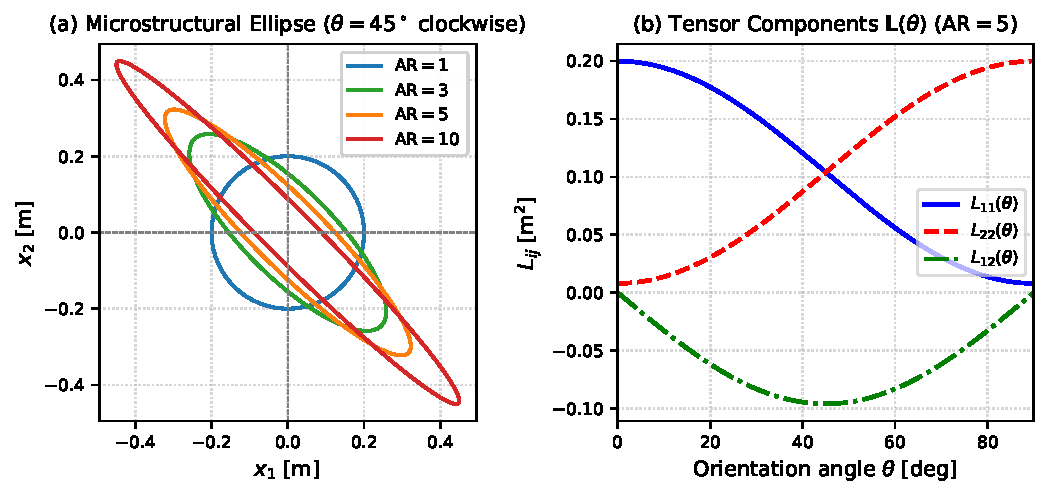
\includegraphics[width=\textwidth]{figures/fig01_ellipsoid_tensor.pdf}
\caption{Length-scale anisotropy. (a) Equal-area ellipses at $\theta=45^\circ$. (b) Length-tensor components against orientation for $\mathrm{AR}=5$.}
\label{fig:ellipsoid_tensor}
\end{figure*}

\subsection{Kinematics and constitutive response}
We assume infinitesimal deformations and two-dimensional plane-strain conditions ($u_3 = 0, \partial(\cdot)/\partial x_3 = 0$). The classical displacement gradient gives the infinitesimal strain tensor $\bm\varepsilon$:
\begin{equation}
\varepsilon_{ij} = \frac{1}{2}(u_{i,j} + u_{j,i}), \quad i,j \in \{1, 2\}.
\label{eq:strain_def}
\end{equation}
The strain-gradient tensor $\bm\eta$ is the spatial derivative of the strain:
\begin{equation}
\eta_{ijk} = \varepsilon_{ij,k} = \frac{1}{2}(u_{i,jk} + u_{j,ik}), \quad \eta_{ijk} = \eta_{jik}.
\label{eq:strain_gradient_def}
\end{equation}
Under plane strain in 2D, $\bm\varepsilon$ has 3 independent components ($\varepsilon_{11}, \varepsilon_{22}, 2\varepsilon_{12}$), and $\bm\eta$ has 6 ($\eta_{111}, \eta_{112}, \eta_{221}, \eta_{222}, 2\eta_{121}, 2\eta_{122}$).

\subsubsection{Mindlin Form-II constitutive law}
In Mindlin's Form II, the strain-energy density $W$ has classical and strain-gradient contributions:
\begin{equation}
W = \frac{1}{2}\sigma_{ij}\varepsilon_{ij} + \frac{1}{2}\tau_{ijk}\eta_{ijk},
\label{eq:strain_energy_W}
\end{equation}
where $\bm\sigma$ is the Cauchy stress tensor and $\bm\tau$ is the third-order double-stress (or dipolar stress) tensor. For an isotropic base material parameterised by the Lam\'e constants $\lambda$ and $\mu$, the Cauchy stress satisfies Hooke's law:
\begin{equation}
\sigma_{ij} = C_{ijkl}\varepsilon_{kl} = \lambda \delta_{ij}\varepsilon_{kk} + 2\mu \varepsilon_{ij}.
\label{eq:cauchy_stress}
\end{equation}
The double-stress tensor $\tau_{ijk}$ is conjugate to $\eta_{ijk}$ through the anisotropic gradient-elasticity law with $\mathbf{L}$:
\begin{equation}
\begin{split}
\tau_{ijk} &= \frac{1}{10} L_{kl} C_{ijmn}\eta_{mnl} \\
&= \frac{1}{10} L_{kl}\left(\lambda \delta_{ij}\eta_{mml} + 2\mu \eta_{ijl}\right),
\end{split}
\label{eq:double_stress}
\end{equation}
For stable isotropic elastic constants ($\mu>0$ and $3\lambda+2\mu>0$) and positive-definite $\mathbf{L}$, the quadratic strain energy is non-negative and vanishes only when the strain and strain-gradient fields both vanish.

\subsubsection{Gradient micro-inertia}
We include gradient micro-inertia in the kinetic-energy density $T$:
\begin{equation}
T = \frac{1}{2}\rho \dot u_i \dot u_i + \frac{1}{2}\rho \ell_{\mathrm{i}}^2 \dot u_{i,j}\dot u_{i,j},
\label{eq:kinetic_energy_T}
\end{equation}
where $\rho$ is the macroscopic mass density and $\ell_{\mathrm{i}} > 0$ is the independent micro-inertia length parameter. Applying Hamilton's principle $\delta \int_{t_1}^{t_2} (T - W)\,\dif t = 0$ gives the strong-form equations of dynamic equilibrium in the bulk:
\begin{equation}
\sigma_{ij,j} - \tau_{ijk,jk} = \rho\left(\ddot u_i - \ell_{\mathrm{i}}^2 \ddot u_{i,jj}\right), \quad \text{in } \Omega.
\label{eq:strong_form}
\end{equation}
The operator $1-\ell_{\mathrm{i}}^2\nabla^2$ increases the effective inertia of spatially varying acceleration. It gives the transverse branch a finite high-wavenumber phase-speed limit, as derived in Appendix~\ref{app:asymptotics}.

\subsubsection{Model reductions}
The model has four useful physical limits:
\begin{enumerate}[label=(\roman*)]
  \item \textbf{Classical elasticity limit ($l_{\mathrm{iso}} \to 0$ at fixed finite $\mathrm{AR}$, $\ell_{\mathrm{i}} \to 0$):} Both principal gradient lengths and the double stresses vanish, and the classical Navier equations $\sigma_{ij,j}=\rho\ddot u_i$ are recovered with dispersionless acoustic speeds $c_T=\sqrt{\mu/\rho}$ and $c_L=\sqrt{(\lambda+2\mu)/\rho}$.
  \item \textbf{Isotropic gradient elasticity ($\mathrm{AR} = 1$):} Here $l_1 = l_2 = l_{\mathrm{iso}}$, so $L_{11} = L_{22} = l_{\mathrm{iso}}^2$ and $L_{12} = 0$ for all $\theta$, recovering isotropic Form-II gradient elasticity.
  \item \textbf{Gradient elasticity without micro-inertia ($\ell_{\mathrm{i}} = 0$):} The higher order stiffness is reserved, while the inertial correction is gone. For the transverse branch, $v_p\propto k$ as $k\to\infty$.
  \item \textbf{Quarter-turn covariance:} For fixed $l_1,l_2$, a $90^\circ$ change of orientation interchanges the diagonal components and reverses the sign of the off-diagonal component: $L_{11}(\theta+90^\circ)=L_{22}(\theta)$, $L_{22}(\theta+90^\circ)=L_{11}(\theta)$, and $L_{12}(\theta+90^\circ)=-L_{12}(\theta)$.
\end{enumerate}

\subsection{Boundary operators}
Suppose that the boundary $\Gamma=\partial\Omega$ is smooth and has the unit outward normal $\bm n$. The boundary contribution comes from the strain-energy term integrated by parts.
\begin{equation}
\begin{split}
\left.\delta\int_\Omega W\,\dif\Omega\right|_\Gamma
={}& \int_\Gamma \Big[(\sigma_{ij}-\tau_{ijk,k})n_j\,\delta u_i \\
&+ \tau_{ijk}n_k\,\delta u_{i,j}\Big] \,\dif\Gamma.
\end{split}
\label{eq:elastic_boundary_work}
\end{equation}
On a smooth boundary, we decompose $\delta u_{i,j}$ into normal and tangential parts. Integrating the tangential part by parts then gives the work-conjugate double traction and the effective elastic traction:
\begin{equation}
\begin{split}
R_i &= n_jn_k\tau_{ijk}, \\
p_i^{\mathrm{el}} &= (\sigma_{ij}-\tau_{ijk,k})n_j - \nabla_j^S(n_k\tau_{ijk}),
\end{split}
\label{eq:traction_def}
\end{equation}
where $\nabla_j^S$ denotes the surface divergence on the tangential component of $n_k\tau_{ijk}$. Additional line forces arise at boundary edges. The gradient micro-inertia adds $\rho\ell_{\mathrm{i}}^2\ddot u_{i,j}n_j$ to the dynamic traction, so $p_i^{\mathrm{dyn}}=p_i^{\mathrm{el}}+\rho\ell_{\mathrm{i}}^2\ddot u_{i,j}n_j$. The work-conjugate pairs are $(u_i,p_i^{\mathrm{dyn}})$ and $(\partial u_i/\partial n,R_i)$. The paired cell faces carry Bloch phase conditions instead of independent free-boundary conditions.

\section{Bloch--Floquet formulation and observables}
\label{sec:bloch}

\subsection{Square lattice and Bloch conditions}
We repeat the square cell $\Omega_{\mathrm{cell}}=[0,L]\times[0,L]$ along the lattice vectors
\begin{equation}
\bm{a}_1=\begin{bmatrix}L \\ 0\end{bmatrix},\qquad
\bm{a}_2=\begin{bmatrix}0 \\ L\end{bmatrix}.
\label{eq:lattice_vectors}
\end{equation}
The corresponding reciprocal vectors satisfy $\bm{a}_i\cdot\bm{b}_j=2\pi\delta_{ij}$:
\begin{equation}
\bm{b}_1=\frac{2\pi}{L}\begin{bmatrix}1\\0\end{bmatrix},\qquad
\bm{b}_2=\frac{2\pi}{L}\begin{bmatrix}0\\1\end{bmatrix}.
\label{eq:reciprocal_vectors}
\end{equation}
The first Brillouin zone is $\mathcal{B}=[-\pi/L,\pi/L]^2$. For the isotropic square lattice, $C_{4v}$ symmetry permits the path $\Gamma(0,0)$--$X(\pi/L,0)$--$M(\pi/L,\pi/L)$--$\Gamma$. For the orientations considered, the symmetry reduces to $C_{2v}$ at $\theta=0^\circ$ and $90^\circ$ and to $C_2$ otherwise. Complete-gap measures use the full Brillouin zone. Figure~\ref{fig:lattice_ibz} shows the periodic square lattice and this high-symmetry $\Gamma$--$X$--$M$--$\Gamma$ contour.

\begin{figure*}[htbp]
\centering
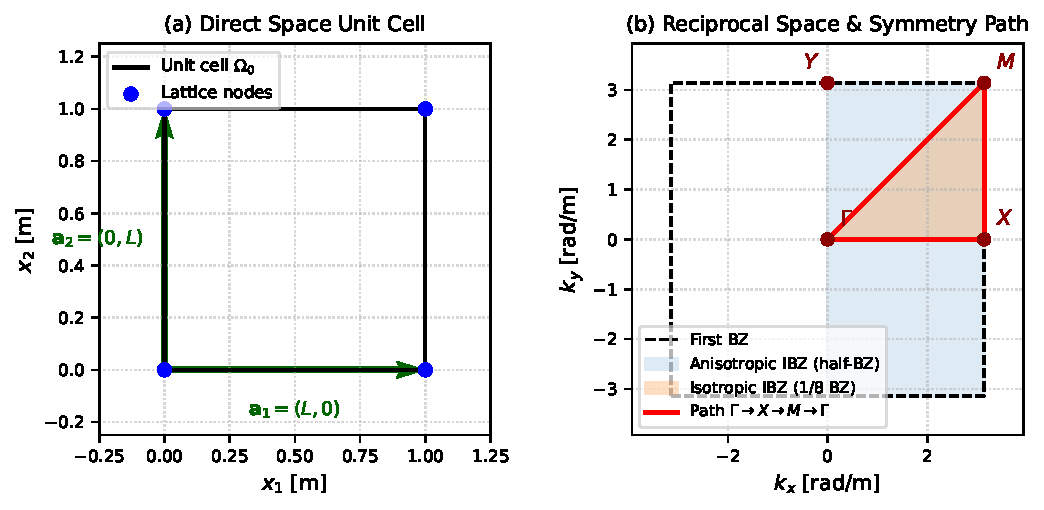
\includegraphics[width=\textwidth]{figures/fig02_lattice_ibz.pdf}
\caption{(a) Square periodic lattice. (b) First Brillouin zone and the high-symmetry contour $\Gamma$--$X$--$M$--$\Gamma$.}
\label{fig:lattice_ibz}
\end{figure*}

For a time-harmonic displacement $\bmu(\bmx,t)=\tilde{\bmu}(\bmx)e^{\iu(\bmk\cdot\bmx-\omega t)}$, Bloch periodicity gives
\begin{equation}
\bmu(\bmx+\bm{a}_\alpha)=\bmu(\bmx)e^{\iu\bmk\cdot\bm{a}_\alpha},\qquad \alpha\in\{1,2\}.
\label{eq:bloch_displacement}
\end{equation}
Because the approximation is $C^1$-conforming, differentiating the displacement relation gives:
\begin{equation}
\begin{split}
\frac{\partial\bmu}{\partial x_\beta}(\bmx+\bm{a}_\alpha)&=\frac{\partial\bmu}{\partial x_\beta}(\bmx)e^{\iu\bmk\cdot\bm{a}_\alpha},\\
\frac{\partial^2\bmu}{\partial x_1\partial x_2}(\bmx+\bm{a}_\alpha)&=\frac{\partial^2\bmu}{\partial x_1\partial x_2}(\bmx)e^{\iu\bmk\cdot\bm{a}_\alpha}.
\end{split}
\label{eq:bloch_derivatives}
\end{equation}
The phase multiplier is the same for displacement, first derivatives and mixed derivatives. Using a different multiplier for derivative degrees of freedom would violate $C^1$ continuity at the cell boundary.

\subsection{Nondimensionalisation}
For Case~H, we scale length, frequency, and velocity with the cell length $L$, shear modulus $\mu$, and density $\rho$:
\begin{equation}
\begin{split}
\bark&=\frac{kL}{\pi},\qquad \barw=\frac{\omega}{\omega_0},\\
\omega_0&=\sqrt{\frac{\mu}{\rho L^2}},\qquad \bar{l}_m=\frac{l_m}{L},\\
\ellbar&=\frac{\ell_{\mathrm{i}}}{L},\qquad \bar{v}_p=\frac{\omega/k}{\sqrt{\mu/\rho}}.
\end{split}
\label{eq:nondim_defs}
\end{equation}
This gives $c_T=1$ and $c_L=\sqrt{(\lambda+2\mu)/\mu}=\sqrt{3}$ for $\lambda/\mu=1$ ($\nu=0.25$). Case~C uses the matrix shear speed and frequency scale specified in Table~\ref{tab:case_params}.

\begin{table*}[htbp]
\begin{center}
\begin{threeparttable}
\tablebodyfont
\caption{Selected material and numbers for Cases H and C and steering analysis.}
\label{tab:case_params}
\begin{tabular}{@{}l p{2.9cm} p{10.8cm}@{}}
\toprule
Case & Quantity & Value \\
\midrule
H & Cell and matrix & $L=1.0\,\mathrm{m}$; $\lambda=\mu=1.0\,\mathrm{Pa}$; $\rho=1.0\,\mathrm{kg/m^3}$ \\
H & Lengths and mesh & $l_{\mathrm{iso}}=0.20\,\mathrm{m}$; $\ell_{\mathrm{i}}=0.20\,\mathrm{m}$; $16\times16$ BFS elements per cell \\
C & Epoxy matrix & $\rho_m=1142\,\mathrm{kg/m^3}$; $\mu_m=1.48\,\mathrm{GPa}$; $\lambda_m=4.57\,\mathrm{GPa}$ \\
C & YBCO inclusion & $\rho_i=6333\,\mathrm{kg/m^3}$; $\mu_i=37.0\,\mathrm{GPa}$; $\lambda_i=95.0\,\mathrm{GPa}$ \\
C & Geometry and length scales & $L=1.0\,\mathrm{m}$; $r_0/L=0.30$; $\ell_m/L=0.10$; $\ell_i/L=0.20$ \\
C & Frequency scale and reported resolution & $c_{t,m}=1138.4\,\mathrm{m/s}$; $\omega_{0,C}=\pi c_{t,m}/L=3576.4\,\mathrm{rad/s}$; $4\times4$ mesh and $21\times21$ zone grid \\
Steering & Acoustic-branch sweep & $\bar{k}=0.5$; $\mathrm{AR}\in\{5,10\}$; $\theta=0^\circ,15^\circ,\ldots,90^\circ$ \\
\bottomrule
\end{tabular}

\end{threeparttable}
\end{center}
\end{table*}

\subsection{Gap and steering measures}
At each wave vector, we order the eigenfrequencies as $\barw_1(\bmk)\le\barw_2(\bmk)\le\cdots$. We distinguish gaps evaluated on one path leg, on the complete high-symmetry path, and on the full Brillouin zone:
\begin{enumerate}[label=(\alph*)]
  \item \textbf{Leg gap:} for bands $n$ and $n+1$, $\Delta[\mathrm{leg}]=\min_{\bmk\in\mathrm{leg}}\barw_{n+1}(\bmk)-\max_{\bmk\in\mathrm{leg}}\barw_n(\bmk)$. Here $\Delta_{GX}$ denotes the $\Gamma$--$X$ leg.
  \item \textbf{Path gap:}
  \begin{equation}
  \Delta_{\mathrm{path}}=\min_{\bmk\in\mathrm{path}}\barw_{n+1}(\bmk)-\max_{\bmk\in\mathrm{path}}\barw_n(\bmk).
  \label{eq:delta_path}
  \end{equation}
  \item \textbf{Complete gap:}
  \begin{equation}
  \Delta_{\mathrm{complete}}=\min_{\bmk\in\mathcal{B}}\barw_{n+1}(\bmk)-\max_{\bmk\in\mathcal{B}}\barw_n(\bmk).
  \label{eq:delta_complete}
  \end{equation}
\end{enumerate}
The three sets are nested, giving the inequality
\begin{equation}
\Delta[\mathrm{leg}]\ge\Delta[\mathrm{path}]\ge\Delta[\mathrm{complete}].
\label{eq:gap_hierarchy}
\end{equation}
A positive leg gap applies to that leg only. In homogeneous Case~H it reflects reduced-zone folding and does not imply physical attenuation. A complete band gap requires $\Delta_{\mathrm{complete}}>0$.

We measure the orientation sensitivity of a directional gap by
\begin{equation}
S_\theta=\frac{\max_\theta\left|\frac{\partial\Delta}{\partial\theta}\right|}{\max_\theta\Delta}\quad[\mathrm{rad}^{-1}].
\label{eq:S_theta_def}
\end{equation}
{\sloppy  We evaluate the angular derivative on the sampled $15^\circ$ orientation grid $\theta\in\{0^\circ,15^\circ,\ldots,90^\circ\}$, with a central difference at interior points and a one-sided difference at the $\theta=0^\circ$ and $90^\circ$ endpoints.\par}.

The group velocity and its angular deviation from the wave vector are
\begin{equation}
\bmv_g=\nabla_{\bmk}\omega.
\label{eq:group_velocity}
\end{equation}
\begin{equation}
\delta=\angle\bmv_g-\angle\bmk.
\label{eq:steering_angle}
\end{equation}

\section{$C^1$ Finite Element Discretisation}
\label{sec:fem}

\subsection{Bogner--Fox--Schmit Bicubic Hermite Element}
The displacement-based Mindlin Form-II weak form requires second derivatives. Standard $C^0$ Lagrange interpolation is therefore insufficient for an $H^2(\Omega)$-conforming formulation. We use the Bogner--Fox--Schmit (BFS) bicubic element, which is $C^1$-conforming on structured rectangular meshes \cite{bfs1965}.

For a rectangular element of dimensions $2a \times 2b$, we interpolate $u_1(x, y)$ and $u_2(x, y)$ independently, using tensor products of one-dimensional cubic Hermite polynomials:
\begin{equation}
u_i(x, y) = \sum_{a=1}^4 \sum_{p=1}^4 N_{a,p}(x, y) d_{i, a, p}^e, \quad i \in \{1, 2\},
\label{eq:bfs_interpolation}
\end{equation}
where $a \in \{1, 2, 3, 4\}$ indexes the four element vertices, and $p \in \{1, 2, 3, 4\}$ denotes the four nodal degrees of freedom per displacement component:
\begin{equation}
\setlength{\arraycolsep}{3.5pt}
\bm{d}_{i, a}^e = \begin{bmatrix} u_i & \frac{\partial u_i}{\partial x} & \frac{\partial u_i}{\partial y} & \frac{\partial^2 u_i}{\partial x \partial y} \end{bmatrix}^\mathsf{T}_{\text{at node } a}.
\label{eq:nodal_dof_vector}
\end{equation}
Each vertex has four degrees of freedom for each displacement component, giving 32 per element. Figure~\ref{fig:bfs_dof} shows their Bloch-phase mapping. All reported band structures and design maps use a uniform mesh of $n \times n = 16 \times 16$ BFS elements per unit cell. This gives $h=L/n=0.0625$ and $8n^2=2048$ independent degrees of freedom per cell. Here $8n^2$ is the count after Bloch reduction. The Case-C mesh data instead use the assembled count $8(N+1)^2$ before reduction.

\begin{figure*}[htbp]
\centering
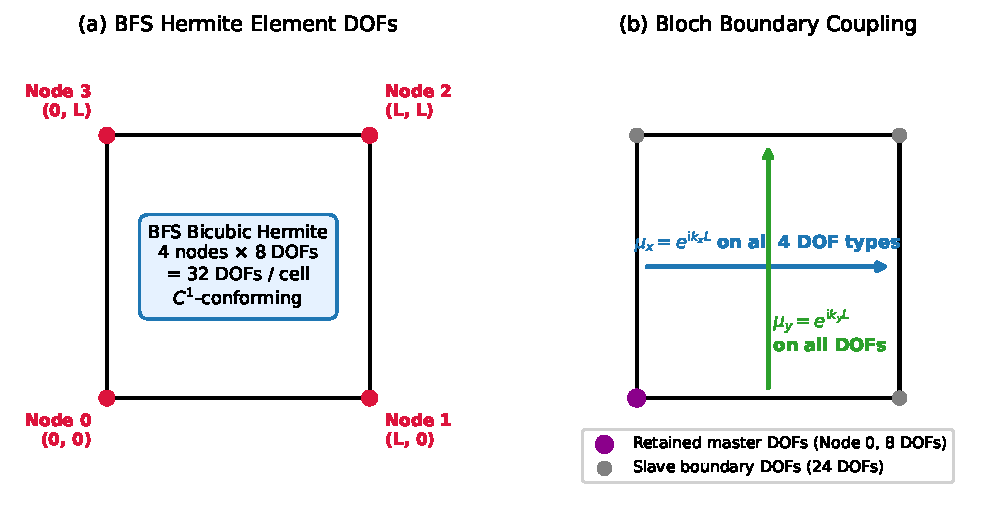
\includegraphics[width=\textwidth]{figures/fig03_bfs_dof_bloch.pdf}
\caption{BFS finite element. (a) Nodal degrees of freedom. (b) Bloch coupling of displacement and derivative degrees of freedom at paired boundaries.}
\label{fig:bfs_dof}
\end{figure*}

\subsection{Element matrices}
The strain tensor $\bm\varepsilon$ and strain-gradient tensor $\bm\eta$ within element $e$ are related to the element nodal displacement vector $\bm{d}^e \in \mathbb{R}^{32}$ through the kinematic strain--displacement matrices $\bmB^c$ and $\bmB^g_k$:
\begin{equation}
\begin{split}
\bm\varepsilon &= \bmB^c \bm{d}^e,\\
\bm\eta_k &\equiv \frac{\partial \bm\varepsilon}{\partial x_k} = \bmB^g_k \bm{d}^e, \quad k \in \{1, 2\}.
\end{split}
\label{eq:strain_matrices}
\end{equation}
The element stiffness matrix $\bmK^e$ has a classical part and a gradient part:
\begin{equation}
\bmK^e = \bmK^c + \bmK^g(\theta, \mathrm{AR}),
\label{eq:Ke_total}
\end{equation}
The classical stiffness matrix is:
\begin{equation}
\bmK^c = \int_{\Omega_e} (\bmB^c)^\mathsf{T} \bmC \bmB^c \,\dif\Omega,
\label{eq:Kc_int}
\end{equation}
The anisotropic gradient stiffness matrix is:
\begin{equation}
\bmK^g(\theta, \mathrm{AR}) = \frac{1}{10} \sum_{k=1}^2 \sum_{l=1}^2 L_{kl}(\theta) \int_{\Omega_e} (\bmB^g_k)^\mathsf{T} \bmC \bmB^g_l \,\dif\Omega.
\label{eq:Kg_int}
\end{equation}
In a homogeneous element, the stiffness and mass integrands have degree at most six in each coordinate. Four Gauss--Legendre points integrate polynomials up to degree seven exactly. A $4\times4$ rule is therefore enough. This avoids quadrature error for homogeneous elements. The unconstrained stiffness still has its expected rigid-body null modes. For elements intersected by the inclusion, we use sub-cell Gauss sampling with an $O(h)$ geometric approximation.

\subsubsection{Mass and micro-inertia matrices}
The kinetic energy gives the classical and micro-inertia mass contributions:
\begin{equation}
\bmM^e = \bmM_0 + \ell_{\mathrm{i}}^2 \bmM^g,
\label{eq:Me_total}
\end{equation}
with:
\begin{equation}
\begin{split}
\bmM_0 &= \rho \int_{\Omega_e} \bm{N}^\mathsf{T} \bm{N} \,\dif\Omega, \\
\bmM^g &= \rho \sum_{k=1}^2 \int_{\Omega_e} \left(\frac{\partial \bm{N}}{\partial x_k}\right)^\mathsf{T} \left(\frac{\partial \bm{N}}{\partial x_k}\right) \,\dif\Omega.
\end{split}
\label{eq:Mg_int}
\end{equation}
Both $\bmM_0$ and $\bmM^g$ are symmetric and positive semi-definite. Their sum $\bmM^e$ is strictly positive definite for any $\rho > 0$.

\subsection{Bloch reduction and eigenproblem}
To impose the Bloch conditions on $\partial\Omega_{\mathrm{cell}}$, we split the global degrees of freedom $\bm{d}$ into interior ($I$), master-boundary ($M$) and slave-boundary ($S$) sets:
\begin{equation}
\bm{d} = \begin{bmatrix} \bm{d}_I \\ \bm{d}_M \\ \bm{d}_S \end{bmatrix}.
\label{eq:d_partition}
\end{equation}
The Bloch transformation links the slave DOFs on the top and right boundaries to the master DOFs on the bottom and left boundaries:
\begin{equation}
\bm{d}_S = \bmT_{SM}(\bmk) \bm{d}_M,
\label{eq:slave_master_rel}
\end{equation}
Here $\bmT_{SM}(\bmk)$ is a diagonal complex phase matrix. Its entries are $e^{\iu k_x L}$, $e^{\iu k_y L}$ or $e^{\iu (k_x + k_y)L}$ for each periodic node pair. Displacement and derivative degrees of freedom share the same phase multiplier.

In the continuous weak form, the natural boundary work cancels between opposite cell faces. The effective traction $p_i^{\mathrm{dyn}}$ carries the Bloch phase and changes sign with the outward normal. Its test trace carries the conjugate phase. The double traction $R_i=n_jn_k\tau_{ijk}$ also carries the Bloch phase, but it keeps its sign when the normal reverses. Its work-conjugate normal derivative changes sign. Together, these signs and phases cancel both face integrals. Line and corner terms pair under the same translations. At the corner, the product phase $e^{\iu(k_x+k_y)L}$ appears. No separate free-boundary condition is imposed on a Bloch-paired face.

We collect these relations in the master--slave transformation matrix $\bmT(\bmk)$:
\begin{equation}
\begin{split}
\bm{d} &= \bmT(\bmk) \bar{\bm{d}}, \quad \bar{\bm{d}} = \begin{bmatrix} \bm{d}_I \\ \bm{d}_M \end{bmatrix}, \\
\bmT(\bmk) &= \begin{bmatrix} \mathbf{I}_{II} & \mathbf{0} \\ \mathbf{0} & \mathbf{I}_{MM} \\ \mathbf{0} & \bmT_{SM}(\bmk) \end{bmatrix},
\end{split}
\label{eq:T_bloch}
\end{equation}
Galerkin projection gives the reduced stiffness and mass matrices:
\begin{equation}
\begin{split}
\bar{\bmK}(\bmk) &= \bmT(\bmk)^\mathsf{H} \bmK \bmT(\bmk), \\
\bar{\bmM}(\bmk) &= \bmT(\bmk)^\mathsf{H} \bmM \bmT(\bmk).
\end{split}
\label{eq:reduced_KM}
\end{equation}

\subsubsection{Reduced Hermitian eigenproblem}
We obtain the dispersion curves $\barw_n(\bmk)$ from the reduced generalised eigenvalue problem:
\begin{equation}
\left[ \bar{\bmK}(\bmk) - \omega^2 \bar{\bmM}(\bmk) \right] \bar{\bm{d}} = \bm{0}.
\label{eq:eigenproblem}
\end{equation}
Each entry of the diagonal phase subblock $\bmT_{SM}(\bmk)$ has unit modulus, so this subblock is unitary. The full matrix $\bmT(\bmk)$ is rectangular with full column rank. Unlike the phase subblock, it is not unitary. For positive elastic and inertial parameters, the full-cell matrices satisfy $\bmK\succeq 0$ and $\bmM\succ 0$. The reduced operators are therefore Hermitian:
\begin{equation}
\begin{split}
\bar{\bmK}(\bmk)^\mathsf{H} &= \bar{\bmK}(\bmk) \succeq 0, \\
\bar{\bmM}(\bmk)^\mathsf{H} &= \bar{\bmM}(\bmk) \succ 0,
\end{split}
\label{eq:hermiticity}
\end{equation}
The generalised eigenvalues $\omega_n^2$ are therefore real and non-negative. Shifting $\bmk$ by a reciprocal-lattice vector $\bm{G}$ leaves every Bloch phase unchanged, so the reduced stiffness and mass matrices satisfy $\bar{\bmK}(\bmk + \bm{G}) = \bar{\bmK}(\bmk)$ and $\bar{\bmM}(\bmk + \bm{G}) = \bar{\bmM}(\bmk)$. The spectrum is periodic across reciprocal space.

\subsubsection{Branch tracking}
Modes of different spatial symmetry can cross along high-symmetry paths. To follow a mode between adjacent wave vectors, we use the Modal Assurance Criterion (MAC) at $\bmk_1$ and $\bmk_2$. Let $\bm{d}_m(\bmk)=\bmT(\bmk)\bar{\bm{d}}_m(\bmk)$ be the full-cell eigenvector. Let $\bmM$ be the common assembled full-cell mass matrix, which includes gradient micro-inertia. The cross-wavevector MAC is
\begin{equation}
{\small
\mathrm{MAC}_{mn}(\bmk_1,\bmk_2) = \frac{\left| \bm{d}_m(\bmk_1)^\mathsf{H} \bmM \bm{d}_n(\bmk_2) \right|^2}{\left( \bm{d}_m(\bmk_1)^\mathsf{H} \bmM \bm{d}_m(\bmk_1) \right) \left( \bm{d}_n(\bmk_2)^\mathsf{H} \bmM \bm{d}_n(\bmk_2) \right)}
}
\label{eq:mac_def}
\end{equation}
The MAC uses the common full-cell mass matrix because the reduced mass matrix depends on $\bmk$. A direct comparison of reduced eigenvectors would therefore be inconsistent. If the off-diagonal MAC indicates a branch exchange, we halve the continuation step. We compute band gaps from the frequency-ordered eigenvalues $\barw_1(\bmk) \le \barw_2(\bmk) \le \dots \le \barw_N(\bmk)$, independently of the mode labels assigned during tracking.

\section{Verification and numerical resolution}
\label{sec:verification}

Verification uses analytical limiting cases, transfer-matrix relations, matrix identities and mesh refinement. The published heterogeneous-bilayer comparisons are more limited: source curves are available only as plots, and some parameter conventions are unclear. We do not use those comparisons as quantitative validation.

\subsection{Analytical limits and bilayer comparison}
In the isotropic homogeneous limit, the long-wavelength phase velocities recover the classical transverse and longitudinal speeds:
\begin{equation}
\begin{split}
\lim_{k\to0}\frac{\omega_T(k)}{k}&=\sqrt{\frac{\mu}{\rho}}=1.0,\\
\lim_{k\to0}\frac{\omega_L(k)}{k}&=\sqrt{\frac{\lambda+2\mu}{\rho}}=\sqrt{3}\approx1.73205.
\end{split}
\label{eq:acoustic_limits}
\end{equation}
At $\bar{k}=0.001$, the computed acoustic speeds differ from these limits by $1.25\times10^{-8}$ (Table~\ref{tab:consistency_suite}). The pure-bending micro-beam reduction matches the published closed-form limits within $10^{-15}$ \cite{papargyribeskou2009}. The micro-inertia asymptote is checked against the analytical result in Appendix~\ref{app:asymptotics}.

As a classical reference, we analyze a periodic AlN/BaTiO$_3$ bilayer with $a_A=a_B=0.01\,\mathrm{m}$ and $b=a_A+a_B=0.02\,\mathrm{m}$ using the Rytov relation \cite{li2024anchorB,zhengwei2009}:
\begin{equation}
\begin{split}
\cos(Kb)={}&\cos(k_Aa_A)\cos(k_Ba_B) \\
&-\frac{1}{2}\left(\frac{Z_A}{Z_B}+\frac{Z_B}{Z_A}\right)\sin(k_Aa_A)\sin(k_Ba_B),
\end{split}
\label{eq:rytov}
\end{equation}
where $k_m=\omega\sqrt{\rho_m/c_{33,m}}$, $v_m=\sqrt{c_{33,m}/\rho_m}$, and $Z_m=\rho_m v_m$. The single-layer transfer-matrix identity and the identical-material bilayer reduction match their analytical limits to $6.47\times10^{-16}$ and $7.22\times10^{-16}$, respectively. The heterogeneous transfer-matrix trace reproduces the Rytov relation to $2.22\times10^{-16}$. The first three calculated stop-band intervals are $[0.4806,0.5209]$, $[0.9812,1.0215]$, and $[1.4993,1.5028]$ in normalized frequency. We compare the result with the published B1 plot visually because tabulated source data are unavailable; no percentage error is inferred from the curves.

We reproduce two gradient-elastic bilayer cases, but do not treat them as external validations. One published length-scale definition is dimensionally ambiguous. For the other, the plotted parameter set and normalization are unspecified, and the numerical curves are unavailable. The parameter interpretations and limitations are documented in Appendix~\ref{app:transfer_checks}. Reproducing the printed dipolar layer matrix checks its algebra, not the published band curves.

\subsection{Numerical consistency and mesh convergence}
Table~\ref{tab:consistency_suite} reports eight checks covering matrix properties, reciprocal-space periodicity, rotational symmetry, acoustic limits, micro-inertia and energy transport. For the energy-flux check, we use closed-form Case-H harmonic fields and the sign convention in Appendix~\ref{app:energy_flux}. The flux-derived velocity agrees with the central-difference group velocity to $6.91\times10^{-10}$ across the tested directions and acoustic branches. The supporting numerical diagnostics are reported in Appendix~\ref{app:numerical_checks}.

Mesh convergence is tested in homogeneous Case~H at $\bmk=(0.31\pi/L,0.22\pi/L)$ using BFS grids with $n=4,8,16$ and $32$ elements per side. Figure~\ref{fig:mesh_convergence} shows the acoustic-frequency error relative to the closed-form value and the change between successive meshes. The first three mesh levels give an empirical rate of $p=4.17$ (95\% CI $[3.15,5.20]$). The $32^2$ result is close to the numerical resolution limit and was omitted from the fit. The fitted rate is not presented as a theoretical convergence order. The measured floor for successive-mesh changes is $\varepsilon_\Delta=4.63\times10^{-11}$; it should not be confused with eigensolver reproducibility. The smallest positive sampled directional separation across the 42-configuration design map, $\Delta_{GX}=1.3\times10^{-3}$ (at $\mathrm{AR}=5$, $\theta=0^\circ$; see Table~\ref{tab:gap_summary}), exceeds the floor by approximately $3\times10^7$.

\begin{figure*}[htbp]
\centering
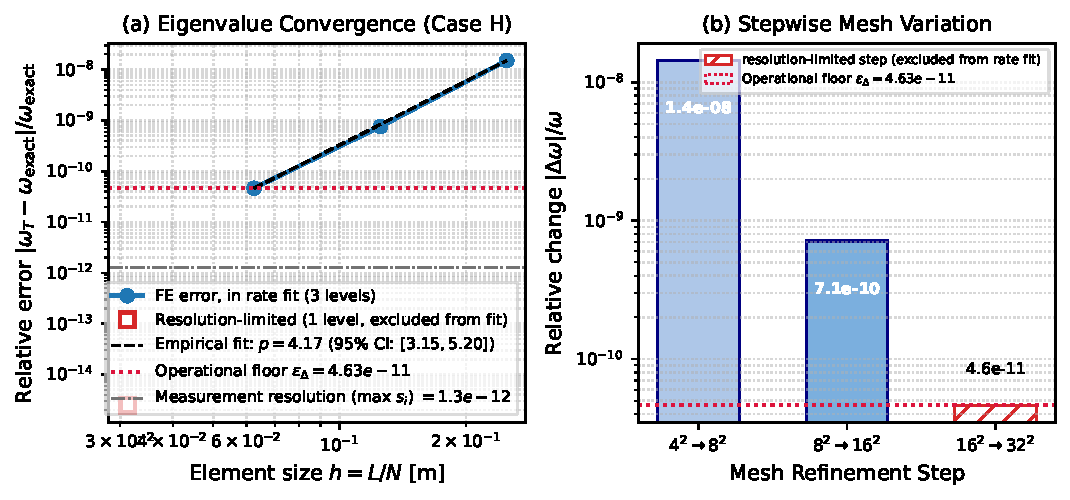
\includegraphics[width=\textwidth]{figures/fig05_mesh_convergence.pdf}
\caption{Case-H mesh convergence. (a) Acoustic-frequency error; the $32^2$ point is excluded from the empirical fit. (b) Successive-mesh changes and numerical floor $\varepsilon_\Delta$.}
\label{fig:mesh_convergence}
\end{figure*}

\begin{table*}[htbp]
\begin{center}
\begin{threeparttable}
\tablebodyfont
\caption{Numerical consistency checks. The energy-flux identity uses closed-form Case-H fields; other checks assess the Bloch finite-element implementation.}
\label{tab:consistency_suite}
\small
\begin{tabular}{@{}p{2.3cm} p{6.9cm} p{2.2cm} c p{1.8cm}@{}}
\toprule
Check & Quantity assessed & Maximum discrepancy & Criterion & Result \\
\midrule
Hermiticity & Reduced stiffness and mass operators & $2.01\times10^{-16}$; $5.63\times10^{-17}$ & $<10^{-12}$ & Within criterion \\
Brillouin-zone periodicity & Spectrum under reciprocal-lattice shifts & $9.66\times10^{-16}$ & $<10^{-10}$ & Within criterion \\
Isotropic rotation & Frequencies at $\mathrm{AR}=1$ & $9.63\times10^{-16}$ & $<10^{-10}$ & Within criterion \\
Acoustic limit & Long-wave transverse and longitudinal slopes & $1.25\times10^{-8}$ & $<10^{-6}$ & Within criterion \\
Rotation--swap symmetry & Spectrum under $\theta\mapsto\theta+90^\circ$ and axis swap & $6.44\times10^{-16}$ & $<10^{-10}$ & Within criterion \\
Definiteness & Two rigid modes at $\Gamma$; positive interior spectrum & As expected & Admissible & As expected \\
Micro-inertia limit & Phase speed at $\bar{k}=200$ versus asymptotic value & $2.85\times10^{-4}$ & $<10^{-3}$ & Within criterion \\
Energy-flux identity (closed-form) & Closed-form group velocity versus cycle-averaged energy flux, Case-H harmonic fields & $6.91\times10^{-10}$ & $<10^{-6}$ & Within criterion \\
\bottomrule
\end{tabular}

\end{threeparttable}
\end{center}
\end{table*}

Additional parameters and convergence data are tabulated in Appendix~\ref{app:extended_checks}.

\section{Results: dispersion, band gaps, and wave steering}
\label{sec:results}

The homogeneous isotropic solid serves as the reference for the orientation and aspect-ratio sweeps. The results then address the periodic composite, group-velocity steering and the high-wavenumber response. Case~H contains no periodic material contrast. Its positive $\Delta_{GX}$ values describe reduced-zone spectral separations, not Bragg attenuation gaps. Case~C contains periodic contrast and is examined separately for complete-gap formation. Unless otherwise stated, every reported Case-H directional and complete-gap measure ($\Delta_{GX}$, $\Delta_{XM}$, $\Delta_{MG}$, $\Delta_{\mathrm{path}}$, $\Delta_{\mathrm{complete}}$) is evaluated on the Bands~2--3 pair. The full parameter set is included in Appendix~\ref{app:parameter_summary}.

\subsection{Homogeneous isotropic baseline}
At $\mathrm{AR}=1$, the principal characteristic lengths coincide and the rotated length tensor is isotropic, so its constitutive response is independent of $\theta$. It therefore provides the reference for the anisotropic calculations, and Figure~\ref{fig:caseH_dispersion} plots its branches alongside theirs; its $\Gamma$--$X$ directional width is $\Delta_{GX}=0.041$.

\subsection{Anisotropy reshapes the Case-H branches}
Figure~\ref{fig:caseH_dispersion} compares the isotropic reference with two orientations of the anisotropic length tensor. Both acoustic branches start at zero frequency at $\Gamma$. Changing aspect ratio and orientation shifts the branches and lifts symmetry-related degeneracies at the zone edge. At $\mathrm{AR}=10$ and $\theta=45^\circ$, a narrow reduced-zone spectral separation appears along $\Gamma$--$X$, with $\Delta_{GX}=0.0043$. Modes propagating in other directions overlap this interval, so it is not a complete gap; the full-zone measure remains $\Delta_{\mathrm{complete}}\le -0.3235$.

In this model, the rotated length tensor changes the gradient-stiffness contribution according to propagation direction. The resulting branch shifts are therefore not uniform across the Brillouin zone: adjacent bands can separate along $\Gamma$--$X$ while modes at other wave vectors remain in the same frequency interval.

\begin{figure*}[htbp]
\centering
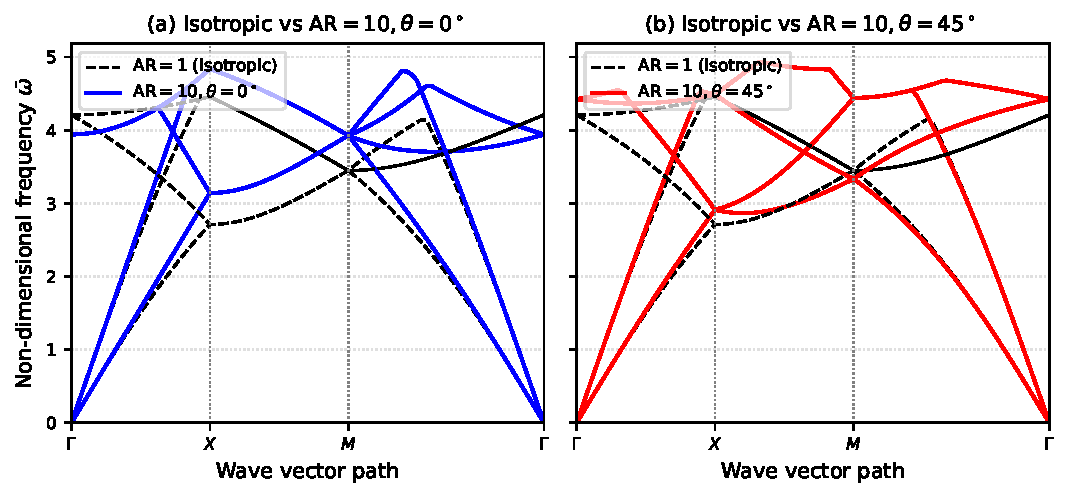
\includegraphics[width=\textwidth]{figures/fig06_caseH_dispersion.pdf}
\caption{Case-H Bloch bands along $\Gamma$--$X$--$M$--$\Gamma$. (a) Isotropic reference ($\mathrm{AR}=1$) and aligned anisotropy ($\mathrm{AR}=10$, $\theta=0^\circ$). (b) Isotropic reference and diagonal anisotropy ($\mathrm{AR}=10$, $\theta=45^\circ$), which opens a narrow $\Gamma$--$X$ reduced-zone spectral separation but no complete gap}
\label{fig:caseH_dispersion}
\end{figure*}

\subsection{Aspect-ratio and orientation effects}
At $\mathrm{AR}=5$, rotating the tensor from $0^\circ$ to $90^\circ$ lowers the transverse frequency at $X$ from $2.915$ to $2.672$ and the longitudinal frequency from $5.050$ to $4.628$ (Figure~\ref{fig:theta_sweep}). The projected gradient length changes from the major to the minor direction. The $M$-point frequencies are symmetric about $45^\circ$, as expected from the square-cell symmetry.

\begin{figure*}[htbp]
\centering
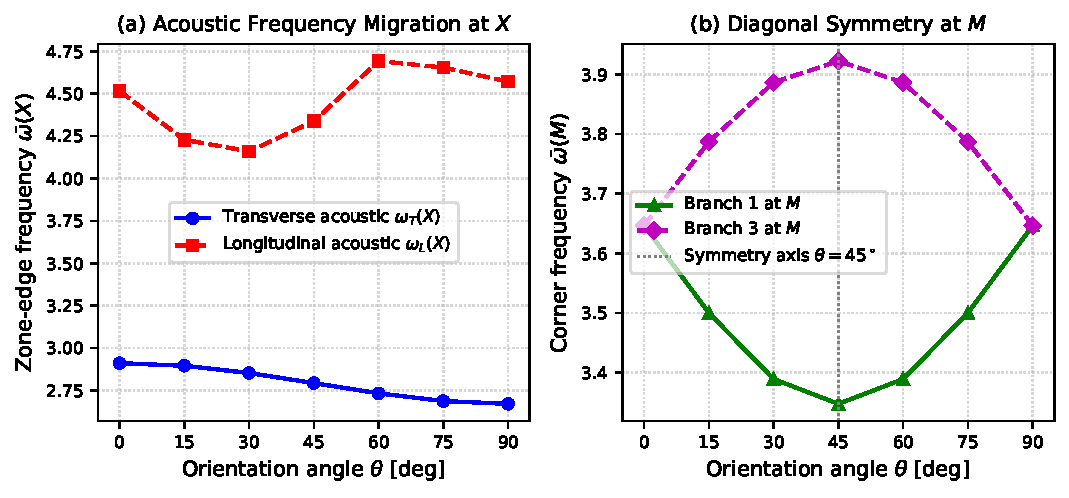
\includegraphics[width=\textwidth]{figures/fig08_theta_sweep.pdf}
\caption{Orientation dependence of the first four Case-H eigenfrequencies at (a) $X$ and (b) $M$ for $\mathrm{AR}=5$. The $M$-point response is symmetric about $\theta=45^\circ$}
\label{fig:theta_sweep}
\end{figure*}

Figure~\ref{fig:ar_sweep} isolates elongation at fixed $\theta=45^\circ$, using volume-equivalent length scaling. At fixed volume-equivalent length, increasing $\mathrm{AR}$ enlarges one principal length and reduces the other. The two band edges consequently respond differently, producing the non-monotone separation seen in the sweep.

\begin{figure*}[htbp]
\centering
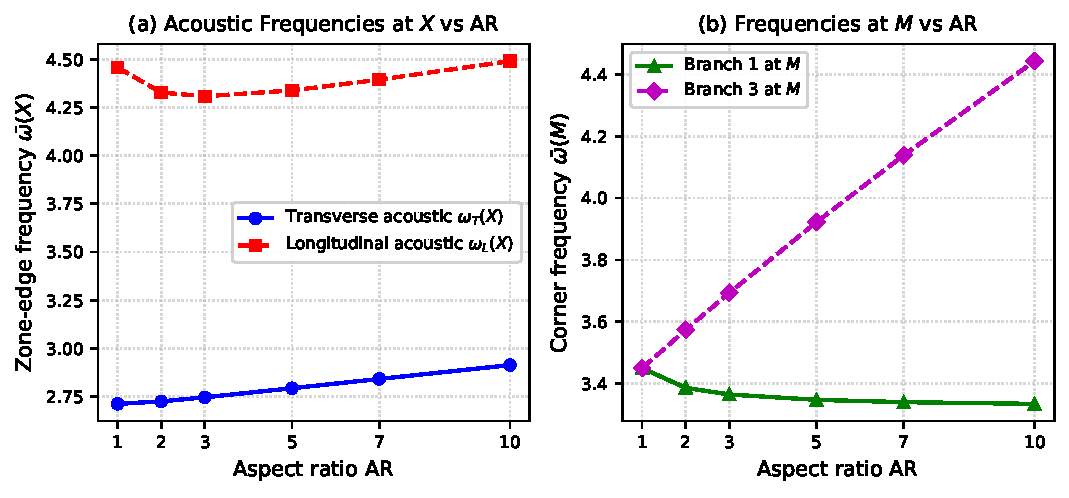
\includegraphics[width=\textwidth]{figures/fig09_ar_sweep.pdf}
\caption{Case-H branch frequencies at $X$ and $M$ as the aspect ratio varies from $1$ to $10$ at fixed $\theta=45^\circ$, using volume-equivalent length scaling}
\label{fig:ar_sweep}
\end{figure*}

\subsection{Directional spectral separation}
The $\Gamma$--$X$ interval is not empty of modes over the entire Brillouin zone. For example, at $\mathrm{AR}=10$ and $\theta=45^\circ$, $\Delta_{GX}=0.0043$ but the complete-gap measure is negative. No homogeneous configuration listed has a complete gap. Table~\ref{tab:gap_summary} lists representative gap measures; mesh-to-mesh variations are given in Appendix~\ref{app:numerical_checks}.

\subsection{Design-map interpretation}
The largest $\Delta_{GX}$ among the 42 sampled designs is $0.0677$ at $(\theta,\mathrm{AR})=(0^\circ,7)$ (Figure~\ref{fig:design_map}). Its dependence on aspect ratio is not monotone. The surface is an interpolation of these designs, not evidence of a continuously optimized configuration. Figure~\ref{fig:polar_map} groups the samples by the sign of $\Delta_{GX}$. The orientation sensitivity $S_\theta$ is largest at $\mathrm{AR}=10$ ($2.34\,\mathrm{rad}^{-1}$).

\begin{figure*}[htbp]
\centering
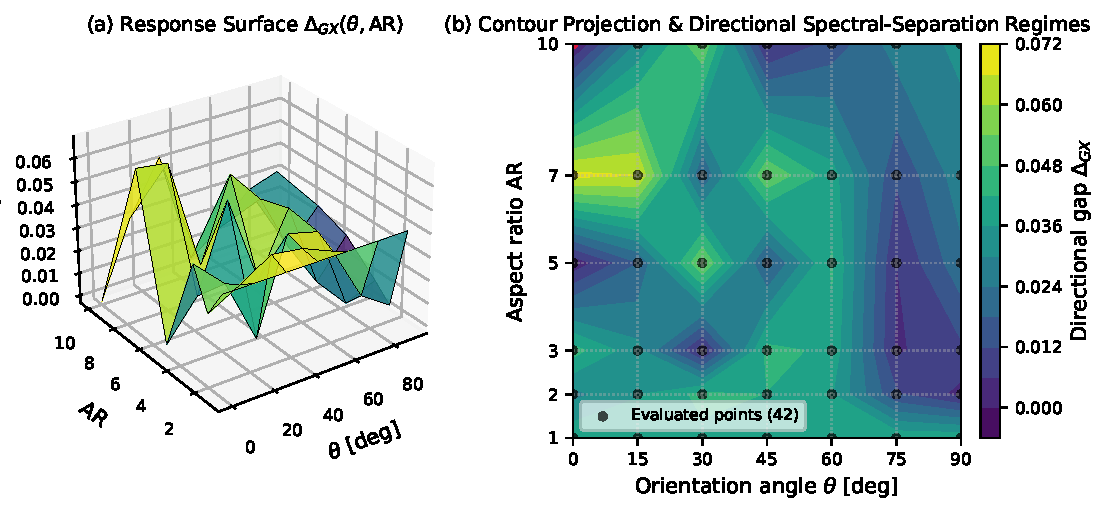
\includegraphics[width=\textwidth]{figures/fig10_design_map_3d.pdf}
\caption{Sampled Case-H design response $\Delta_{GX}(\theta,\mathrm{AR})$ for 42 configurations. The largest sampled value is $0.0677$ at $\theta=0^\circ$, $\mathrm{AR}=7$; at $\theta=45^\circ$, $\mathrm{AR}=10$, $\Delta_{GX}=0.0043$}
\label{fig:design_map}
\end{figure*}

\begin{figure*}[htbp]
\centering
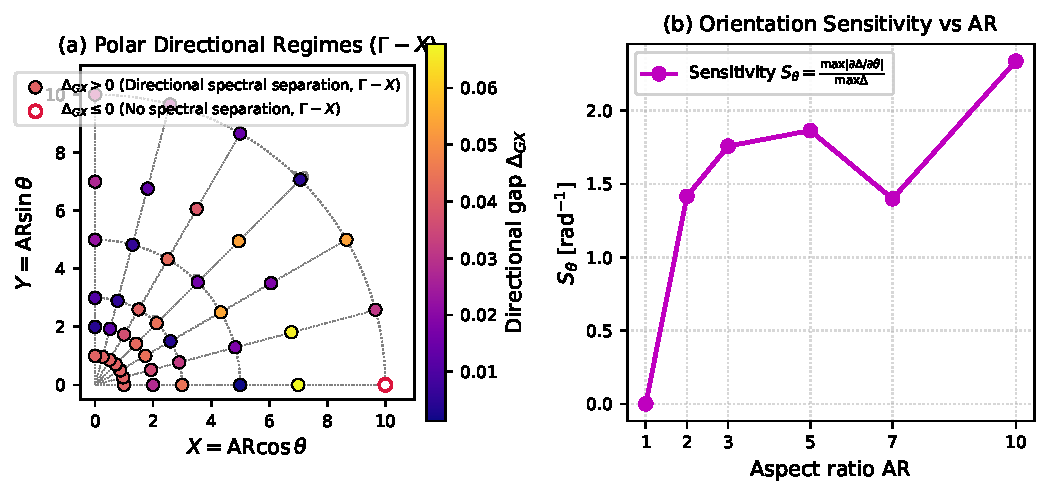
\includegraphics[width=\textwidth]{figures/fig11_polar_map_regimes.pdf}
\caption{Polar-coordinate view of the sampled Case-H designs, classified by $\Delta_{GX}\le0$ (pass band) and $\Delta_{GX}>0$ (directional spectral separation). The displayed boundary is a visual summary of sampled points}
\label{fig:polar_map}
\end{figure*}

\begin{table}[htbp]
\centering
\caption{Directional and complete-gap measures for representative Case-H configurations; values are reported at the precision retained between the $8\times8$ and $16\times16$ meshes}
\label{tab:gap_summary}
\begin{tabular*}{\textwidth}{@{\extracolsep{\fill}}c c r r r@{}}
\toprule
$\mathrm{AR}$ & $\theta$ & $\Delta_{GX}$ & $\Delta_{\mathrm{path}}$ & $\Delta_{\mathrm{complete}}$ \\
\midrule
$1$ & $0^\circ$  & $+0.041$ & $-0.32$ & $-0.32$ \\
$1$ & $45^\circ$ & $+0.041$ & $-0.32$ & $-0.32$ \\
$1$ & $90^\circ$ & $+0.041$ & $-0.32$ & $-0.32$ \\
$3$ & $0^\circ$  & $+0.045$ & $-0.10$ & $-0.46$ \\
$3$ & $45^\circ$ & $+0.044$ & $-0.45$ & $-0.48$ \\
$3$ & $90^\circ$ & $+0.011$ & $-0.33$ & $-0.46$ \\
$5$ & $0^\circ$  & $+0.001$ & $-0.01$ & $-0.58$ \\
$5$ & $45^\circ$ & $+0.016$ & $-0.48$ & $-0.58$ \\
$5$ & $90^\circ$ & $+0.022$ & $-0.37$ & $-0.58$ \\
$10$ & $0^\circ$  & $-0.002$ & $-0.24$ & $-0.85$ \\
$10$ & $45^\circ$ & $+0.004$ & $-0.29$ & $-0.56$ \\
$10$ & $90^\circ$ & $+0.031$ & $-0.65$ & $-0.85$ \\
\bottomrule
\end{tabular*}
\par\vspace{2pt}\begin{minipage}{\textwidth}\footnotesize $S_\theta$ [rad$^{-1}$]: AR $=1$: $0.00$; $2$: $1.42$; $3$: $1.76$; $5$: $1.86$; $7$: $1.40$; $10$: $2.34$.\end{minipage}

\end{table}

\subsection{Heterogeneous Case C: complete gap with periodic contrast}
\label{sec:caseC_pc}
Case~C uses an epoxy--YBCO periodic cell with contrasts $\chi_\mu=25.0$ and $\chi_\rho=5.546$ (Table~\ref{tab:case_params}). We denote the cell period by $L$ in the text and $a$ in Figure~\ref{fig:caseC_dispersion}; $r_0/L=r_0/a=0.30$ gives a filling fraction of $28.27\%$. The circular interface is integrated by sub-cell Gauss sampling on the Cartesian mesh. Figure~\ref{fig:caseC_dispersion} shows a complete gap between Bands~3 and~4 over $\bar{\omega}\in[4.5698,7.1430]$. On the $4\times4$ mesh and $21\times21$ Brillouin-zone grid, $\Delta_{\mathrm{complete}}=2.5732$, or $43.94\%$. Refining the Brillouin-zone grid changes this width by less than $4\times10^{-4}$. Mesh refinement has a substantially larger effect.

\begin{figure*}[htbp]
\centering
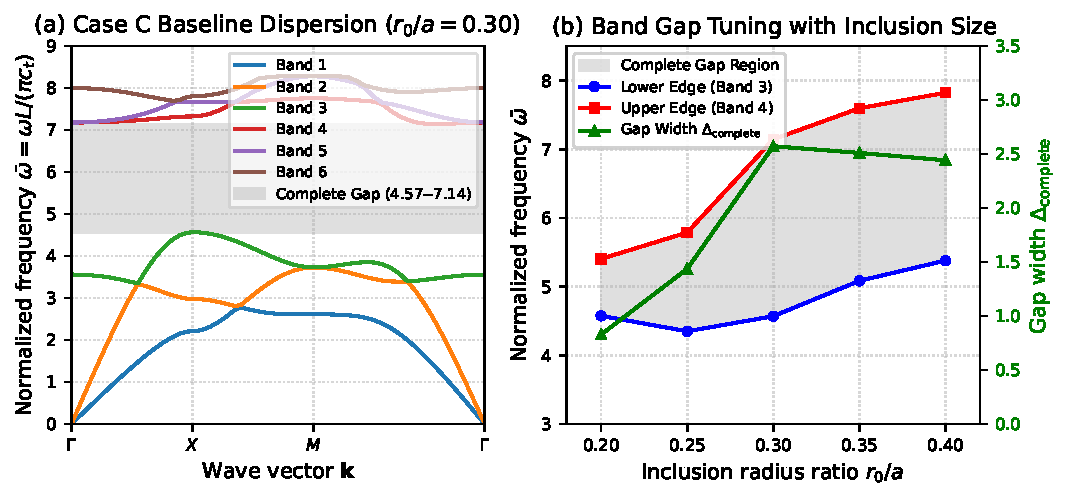
\includegraphics[width=\textwidth]{figures/fig07_caseC_dispersion.pdf}
\caption{Case-C dispersion on the $4\times4$ mesh. (a) Bands~3--4 gap at $r_0/L=0.30$. (b) Gap width versus inclusion radius. The width is not mesh-converged.}
\label{fig:caseC_dispersion}
\end{figure*}

Under mesh refinement, the complete gap falls from $2.5732$ at $4\times4$ to $2.2504$, $2.0722$, $1.9736$, and $1.9179$ at $8\times8$, $16\times16$, $32\times32$, and $64\times64$, respectively. The gap remains open on all five meshes, but its width has not converged. In particular, $2.5732$ describes the $4\times4$ calculation, not the continuum limit. At the $4\times4$ mesh, increasing $r_0/L$ from $0.20$ to $0.30$ widens the gap from $0.8288$ ($16.61\%$) to $2.5732$ ($43.94\%$); it then narrows to $2.4426$ ($37.00\%$) at $r_0/L=0.40$. Mesh and Brillouin-zone sampling details are reported in Appendix~\ref{app:caseC_resolution}.

\subsection{Group-velocity steering}
\label{sec:steering}
On the constant-wavenumber ring $|\bmk|=\bar{k}=0.5$, anisotropy makes the group velocity non-collinear with the wave vector. Group velocity is normal to the local constant-frequency contour because $\bmv_g=\nabla_{\bmk}\omega$. Its angle relative to $\bmk$ therefore depends on the contour slope. Figure~\ref{fig:ifc_wave_steering} plots the angular deviation $\delta(\phi)=\angle\bmv_g-\angle\bmk$ and group-velocity magnitude at $\theta=45^\circ$. The peak deviation rises from $0^\circ$ at $\mathrm{AR}=1$ to $1.4146^\circ$ at $\mathrm{AR}=5$ and $2.7846^\circ$ at $\mathrm{AR}=10$. The magnitude $|\bmv_g|$ also varies around the contour, so the anisotropic dispersion changes the energy-transport speed as well as its direction.

\begin{figure*}[htbp]
\centering
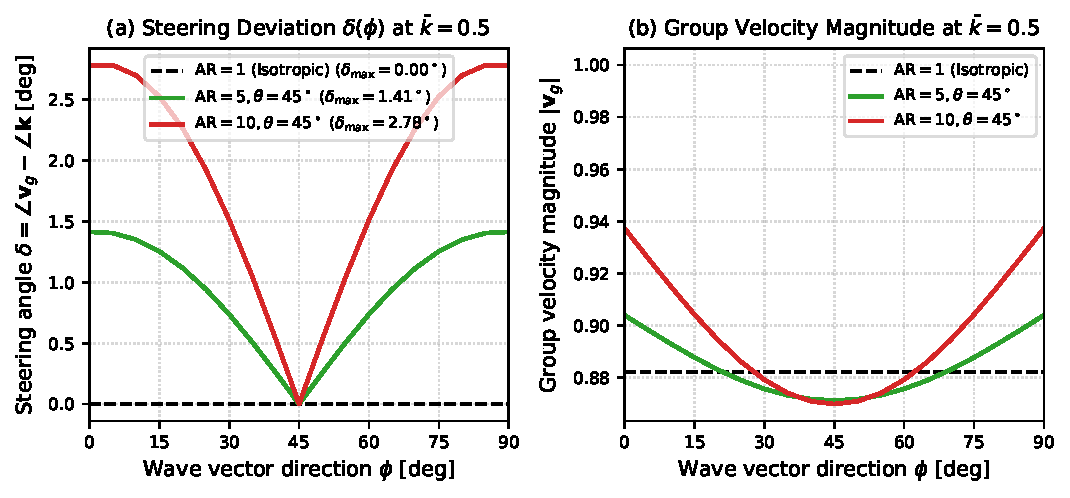
\includegraphics[width=\textwidth]{figures/fig12_ifc_wave_steering.pdf}
\caption{Acoustic-branch group-velocity steering on $|\bmk|=0.5$ at $\theta=45^\circ$. (a) Angular deviation for $\mathrm{AR}=1,5,10$, with peak values $0^\circ$, $1.4146^\circ$, and $2.7846^\circ$. (b) Directional variation of group-velocity magnitude}
\label{fig:ifc_wave_steering}
\end{figure*}

The orientation sweep uses $\theta=0^\circ,15^\circ,\ldots,90^\circ$ at $\mathrm{AR}=5$ and $10$ (Figure~\ref{fig:s7_steering_sweep}; Table~\ref{tab:steering_sweep}). Directions on the wavenumber ring are sampled every $5^\circ$, and a local parabola refines the estimated peak. The refined peaks vary by less than $10^{-5}\,$deg around $1.4146^\circ$ and $2.7846^\circ$, respectively. This small variation reflects the numerical procedure; it should not be interpreted as physical angular accuracy to $10^{-5}$ degrees. The principal direction follows $\phi^*(\theta)\simeq(45^\circ-\theta)\bmod90^\circ$; at $\mathrm{AR}=10$, its excursions are at most $5^\circ$. For the branch and wavenumber ring examined, tensor rotation mainly changes the steering direction. It has little effect on the sampled maximum deviation.

\begin{figure*}[htbp]
\centering
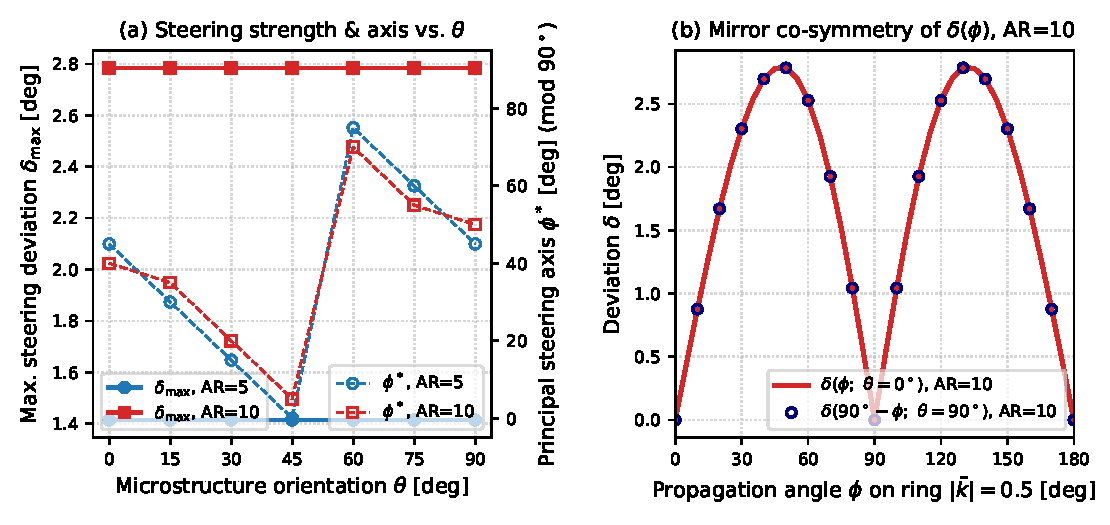
\includegraphics[width=\textwidth]{figures/fig14_s7_steering_sweep.pdf}
\caption{Orientation-dependent steering on $|\bmk|=0.5$. (a) Peak deviation and lobe direction for $\mathrm{AR}=5,10$. (b) Mirrored deviation fields at $\theta=0^\circ$ and $90^\circ$.}
\label{fig:s7_steering_sweep}
\end{figure*}

\begin{table}[htbp]
\centering
\caption{Peak group-velocity deviation and principal steering direction across the sampled orientations at $\bar{k}=0.5$}
\label{tab:steering_sweep}
\setlength{\tabcolsep}{4.5pt}%
\begin{tabular*}{\textwidth}{@{\extracolsep{\fill}}c r r r r@{}}
\toprule
$\theta$ & \multicolumn{2}{c}{$\mathrm{AR}=5$} & \multicolumn{2}{c}{$\mathrm{AR}=10$} \\
\cmidrule(lr){2-3}\cmidrule(lr){4-5}
 & $\delta_{\max}$ [deg] & $\phi^*$ [deg] & $\delta_{\max}$ [deg] & $\phi^*$ [deg] \\
\midrule
$0^\circ$ & 1.4146 & 45 & 2.7846 & 40 \\
$15^\circ$ & 1.4146 & 30 & 2.7846 & 35 \\
$30^\circ$ & 1.4146 & 15 & 2.7846 & 20 \\
$45^\circ$ & 1.4146 & 0 & 2.7846 & 5 \\
$60^\circ$ & 1.4146 & 75 & 2.7846 & 70 \\
$75^\circ$ & 1.4146 & 60 & 2.7846 & 55 \\
$90^\circ$ & 1.4146 & 45 & 2.7846 & 50 \\
\bottomrule
\end{tabular*}
\par\vspace{2pt}\begin{minipage}{\textwidth}\footnotesize $M_s=\phi^*(90^\circ)-\phi^*(0^\circ)$: $M_s(\mathrm{AR}=5)=0^\circ$ and $M_s(\mathrm{AR}=10)=10^\circ$. The $5^\circ$ ring-sampling step limits the resolution of this difference; parabolic peak refinement remains within one sampling step.\end{minipage}
\par\vspace{2pt}\begin{minipage}{\textwidth}\footnotesize Headless periodicity and mirror co-symmetry residuals are each $\le1.3\times10^{-6}\,$deg: $\delta(\phi;\theta)=\delta(\phi+180^\circ;\theta)$ and $\delta(\phi;\theta)=\delta(90^\circ-\phi;90^\circ-\theta)$.\end{minipage}

\end{table}

We define the sampled steering measure as follows:
\begin{equation}
M_s(\mathrm{AR})=\phi^*(90^\circ,\mathrm{AR})-\phi^*(0^\circ,\mathrm{AR}),
\label{eq:Ms_def}
\end{equation}
For the two aspect ratios, the values are:
\begin{equation}
M_s(\mathrm{AR}=5)=0^\circ,\qquad M_s(\mathrm{AR}=10)=10^\circ.
\label{eq:Ms_value}
\end{equation}
The $5^\circ$ ring-sampling step sets the resolution of this difference. The deviation field is headless-periodic and mirror co-symmetric, with residuals no greater than $1.3\times10^{-6}\,$deg. The peak amplitude is invariant under $\theta\mapsto90^\circ-\theta$ to within $10^{-7}\,$deg. These symmetries are consistent with orientation shifting the lobes while leaving the sampled peak deviation unchanged.

\section{Gradient micro-inertia and the high-wavenumber response}
\label{sec:microinertia}

Gradient micro-inertia accounts for spatial gradients of velocity in the kinetic energy. We examine the resulting high-wavenumber behaviour of the transverse branch and the associated strain-energy partition.

\subsection{Energy partition and the transverse-branch limit}
For Mindlin Form-II elasticity, the strain energy splits into classical and gradient parts, $W=W_c+W_g$, with $W_c=\tfrac12\int_\Omega\sigma_{ij}\varepsilon_{ij}\,\dif\Omega$ and $W_g=\tfrac12\int_\Omega\tau_{ijk}\eta_{ijk}\,\dif\Omega$. Along $\Gamma$--$X$, the gradient-energy fraction rises from $0.20\%$ at $\bar{k}=0.1$ to $16.49\%$ at $\bar{k}=1.0$ (Figure~\ref{fig:energy_microinertia}). The contribution of double-stress work increases as the wavelength becomes shorter.

\begin{figure*}[htbp]
\centering
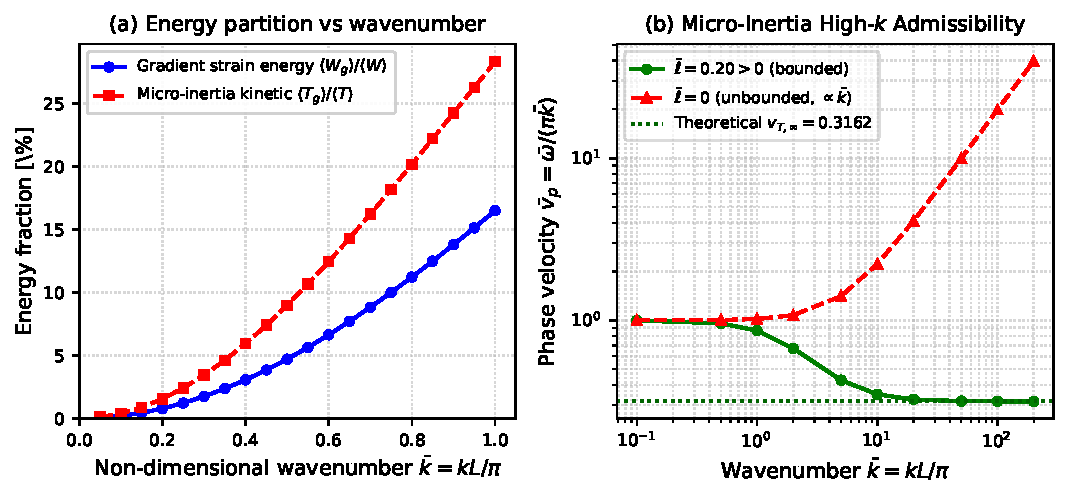
\includegraphics[width=\textwidth]{figures/fig13_energy_microinertia.pdf}
\caption{(a) Gradient-energy fraction $W_g/W$ versus wavenumber. (b) Transverse-branch phase velocity with and without gradient micro-inertia; the finite high-wavenumber limit is specific to the shear branch analyzed here}
\label{fig:energy_microinertia}
\end{figure*}

The transverse shear branch analyzed in Appendix~\ref{app:asymptotics} has the asymptotic limit
\begin{equation}
\begin{split}
\bar{v}_{T,\infty} &= \frac{\bar{l}_{\mathrm{eff}}}{\sqrt{10}\,\bar{\ell}_{\mathrm{i}}} \\
&= \frac{0.20}{\sqrt{10}\times0.20} = \frac{1}{\sqrt{10}} \approx 0.3162.
\end{split}
\label{eq:v_horizon_sec7}
\end{equation}
At $\bar{k}=200$, the computed phase speed with micro-inertia is $0.3163$, within $0.03\%$ of this asymptote. Without micro-inertia, the analytical branch relation grows without bound, and the computed phase speed reaches $39.75$ at $\bar{k}=200$. In Eq.~\eqref{eq:appA_vp}, the gradient stiffness and micro-inertia terms scale with $k^2$ in the numerator and denominator of $v_p^2$. Their ratio approaches a finite value. When $\ell_{\mathrm{i}}=0$, that denominator correction vanishes and the phase speed increases without bound. This result applies only to the transverse branch and constitutive model studied; it does not establish a speed bound for other branches or models.

\section{Discussion and limitations}
\label{sec:discussion}

The directional separations in Case~H are due to the anisotropic gradient stiffness of a homogeneous continuum. At fixed volume-equivalent length, a change in aspect ratio shifts the two bounding frequencies by different amounts. The propagation directions that are most affected are different when the rotation is changed. Where $\Delta_{GX}>0$ the complete-gap measure is negative $\Delta_{\mathrm{complete}}\le -0.3235$. There is no material contrast, and the 42 configurations form a finite design grid. The results are for reduced-zone dispersion. They are not about a Bragg attenuation gap or continuous optimized design.

Another expression of the same anisotropy is obtained from the group velocity calculation. In the acoustic branch at $\bar{k}=0.5$ rotation causes the steering lobes to rotate about the constant-wavenumber ring. Their maximum angular deviation is not significantly affected. The local normal to a contour of constant frequency, $\bmv_g$, is equal to $\nabla_{\bmk}\omega$. This direction need not coincide with $\bmk$, and this is the origin of the computed steering. The result holds for the branch and wavenumber ring tested.

The case~C is different, since its shear modulus and density are periodically changing. Bands~3 and~4 stay separated over the sampled Brillouin zone. The complete-gap width falls from $2.5732$ on the $4\times4$ mesh to $1.9179$ on the $64\times64$ mesh. Further mesh refinement is needed before the width can be taken as a continuum value. There are differences between the homogeneous and composite cases too in their material and numerical settings. The comparison thus reveals two mechanisms. It does not single out one parameter.

Numerical checks support the implementation within these limits. The empirical rate of the homogeneous mesh study is $p=4.17$ for the first three resolutions and the result at $32^2$ is at the numerical floor. There are 8 consistency checks that meet their criteria. One of them is the closed-form Case-H residual of energy-flux, $6.91\times10^{-10}$. The classical relation between AlN and BaTiO$_3$ transfer matrix agrees to $2.22\times10^{-16}$. The comparisons with published bilayer band plots remain qualitative due to the absence of source data or conventions for the parameters. For the transverse-branch asymptotics, the micro-inertia term balances the gradient-stiffness term and gives a finite phase speed at high wavenumber. The other branches are not included in this result. The continuum model is linear, local, isothermal and two dimensional. Dissipation, nonlinear effects, piezoelectric coupling and three-dimensional polarisation modes are not included.
\section{Conclusions}
\label{sec:conclusions}

The main findings from the two-dimensional Mindlin Form-II Bloch-wave calculations are:

\begin{itemize}
  \item The conforming Bogner--Fox--Schmit element imposes consistent Bloch phases on displacement and derivative degrees of freedom. Analytical limits and numerical checks support the implementation.

  \item In homogeneous Case~H, tensor orientation and aspect ratio shift the dispersion branches. Directional reduced-zone separations occur, but no complete band gap is found.

  \item At fixed ellipse area, the separation varies non-monotonically with aspect ratio. The largest sampled value is $\Delta_{GX}=0.0677$ at $\theta=0^\circ$ and $\mathrm{AR}=7$.

  \item Rotating the length tensor changes the direction of acoustic energy flow. The peak group-velocity deviation reaches about $2.78^\circ$, with little change in its magnitude across the sampled orientations.

  \item The periodic epoxy--YBCO composite exhibits a gap between Bands~3 and~4 on all computed meshes. Its width decreases under refinement and remains unconverged.

  \item Gradient micro-inertia limits the high-wavenumber phase speed of the transverse branch to $0.3162$ in normalized units. Without micro-inertia, the corresponding phase speed grows without bound.
\end{itemize}

These results are relevant to the modelling of direction-dependent elastic-wave transport in microstructured solids and to the design of phononic media with controlled wave steering. The homogeneous model provides a means of examining orientation effects without periodic material contrast, while the composite calculations address band-gap formation. Practical use would require material-specific calibration and further convergence checks for the composite gap.

\section*{Declaration of competing interest}
The author declares no competing financial or non-financial interests.
\appendix
% Elsarticle otherwise produces 'Appendix Appendix A' in explicit prose.
\renewcommand{\thesection}{\Alph{section}}
\section{High-Wavenumber Phase Velocity Asymptotics}
\label{app:asymptotics}

We derive the high-wavenumber phase-speed limit for the one-dimensional transverse-shear branch of the strain-gradient model. Without micro-inertia ($\ell_{\mathrm{i}}=0$), the phase velocity grows without bound as $k\to\infty$. With micro-inertia ($\ell_{\mathrm{i}}>0$), it approaches a finite asymptote.

We consider one-dimensional transverse-shear propagation in a Mindlin Form-II gradient-elastic continuum governed by the equation of motion:
\begin{equation}
\begin{split}
\mu \frac{\partial^2 u}{\partial x^2} - \frac{1}{10} \mu l_{\mathrm{eff}}^2 \frac{\partial^4 u}{\partial x^4}
&= \rho \frac{\partial^2 u}{\partial t^2} - \rho \ell_{\mathrm{i}}^2 \frac{\partial^4 u}{\partial x^2 \partial t^2},
\end{split}
\label{eq:appA_pde}
\end{equation}
where $\mu$ is the shear modulus, $\rho$ is the mass density, $l_{\mathrm{eff}}^2 = \hat{\bmk}\cdot\mathbf{L}\cdot\hat{\bmk}$ is the effective characteristic gradient-stiffness length scale (with the factor $1/10$ inherited from the second moment of the 3D ellipsoidal domain), and $\ell_{\mathrm{i}}$ is the micro-inertia length parameter. Substituting the time-harmonic plane wave ansatz $u(x, t) = A e^{\iu(k x - \omega t)}$ into Eq.~\eqref{eq:appA_pde} gives:
\begin{equation}
-\mu k^2 - \frac{1}{10} \mu l_{\mathrm{eff}}^2 k^4 = -\rho \omega^2 - \rho \ell_{\mathrm{i}}^2 \omega^2 k^2.
\label{eq:appA_char}
\end{equation}
Solving this equation gives the dispersion relation:
\begin{equation}
\omega^2(k) = \frac{\mu}{\rho} \frac{k^2 \left( 1 + \frac{1}{10} l_{\mathrm{eff}}^2 k^2 \right)}{1 + \ell_{\mathrm{i}}^2 k^2}.
\label{eq:appA_dispersion}
\end{equation}
The phase velocity $v_p(k) \equiv \omega(k)/k$ is therefore:
\begin{equation}
\begin{split}
v_p(k) &= \sqrt{\frac{\mu}{\rho}} \sqrt{\frac{1 + \frac{1}{10} l_{\mathrm{eff}}^2 k^2}{1 + \ell_{\mathrm{i}}^2 k^2}} \\
&= c_T \sqrt{\frac{1 + \frac{1}{10} l_{\mathrm{eff}}^2 k^2}{1 + \ell_{\mathrm{i}}^2 k^2}},
\end{split}
\label{eq:appA_vp}
\end{equation}
where $c_T = \sqrt{\mu/\rho}$ is the classical acoustic shear wave speed.

\subsection{Case 1: No micro-inertia ($\ell_{\mathrm{i}} = 0$)}
Setting $\ell_{\mathrm{i}} = 0$ in Eq.~\eqref{eq:appA_vp} gives:
\begin{equation}
v_p(k) = c_T \sqrt{1 + \frac{1}{10} l_{\mathrm{eff}}^2 k^2}.
\label{eq:appA_vp_zero}
\end{equation}
In the short-wave limit ($k \to \infty$), the phase velocity behaves asymptotically as:
\begin{equation}
\lim_{k \to \infty} v_p(k) = \lim_{k \to \infty} \frac{c_T l_{\mathrm{eff}}}{\sqrt{10}} k \to \infty.
\label{eq:appA_unbounded}
\end{equation}
The group velocity $v_g(k) = \dif\omega/\dif k$ is:
\begin{equation}
\begin{split}
v_g(k) &= c_T \frac{1 + \frac{2}{10} l_{\mathrm{eff}}^2 k^2}{\sqrt{1 + \frac{1}{10} l_{\mathrm{eff}}^2 k^2}} \\
&\sim \frac{2 c_T l_{\mathrm{eff}}}{\sqrt{10}} k \to \infty \quad \text{as } k \to \infty.
\end{split}
\label{eq:appA_vg_unbounded}
\end{equation}
Both phase and group velocities are therefore unbounded at high wavenumbers in this one-dimensional transverse-shear model when micro-inertia is omitted.

\subsection{Case 2: With micro-inertia ($\ell_{\mathrm{i}} > 0$)}
For $\ell_{\mathrm{i}} > 0$, taking the limit of Eq.~\eqref{eq:appA_vp} as $k \to \infty$ gives:
\begin{equation}
\begin{split}
v_{p,\infty} \equiv \lim_{k \to \infty} v_p(k)
&= c_T \lim_{k \to \infty} \sqrt{\frac{\frac{1}{10} l_{\mathrm{eff}}^2 k^2 (1 + \frac{10}{l_{\mathrm{eff}}^2 k^2})}{\ell_{\mathrm{i}}^2 k^2 (1 + \frac{1}{\ell_{\mathrm{i}}^2 k^2})}} \\
&= c_T \frac{l_{\mathrm{eff}}}{\sqrt{10}\,\ell_{\mathrm{i}}}.
\end{split}
\label{eq:appA_vp_bounded}
\end{equation}
With velocity scaled by $c_T = 1.0$, the dimensionless limit is:
\begin{equation}
\bar{v}_{T,\infty} = \frac{\bar{l}_{\mathrm{eff}}}{\sqrt{10}\,\bar{\ell}_{\mathrm{i}}}.
\label{eq:appA_v_horizon}
\end{equation}
For the Case H baseline ($l_{\mathrm{eff}} = l_{\mathrm{iso}} = 0.20\,\mathrm{m}$, $\ell_{\mathrm{i}} = 0.20\,\mathrm{m}$ from Table~\ref{tab:case_params}, with $\bar{l}_{\mathrm{eff}} = 0.20$ and $\bar{\ell}_{\mathrm{i}} = 0.20$), the transverse asymptotic limit is:
\begin{equation}
\bar{v}_{T,\infty} = \frac{0.20}{\sqrt{10} \times 0.20} = \frac{1}{\sqrt{10}} \approx 0.3162.
\label{eq:appA_horizon_val}
\end{equation}
As verified numerically in Section~\ref{sec:microinertia}, the finite-element phase velocity at $\bar{k} = 200$ reaches $\bar{v}_p = 0.3163$, matching the analytical limit within $0.03\%$. For this transverse branch, micro-inertia gives a finite high-wavenumber phase-speed limit.

\section{Time-Averaged Energy Flux in Form-II Gradient Elasticity}
\label{app:energy_flux}

The energy balance and cycle-averaged mechanical flux are derived here for the Mindlin Form-II solid with gradient micro-inertia.

The local balance of mechanical energy is expressed by the continuity relation:
\begin{equation}
\frac{\partial}{\partial t}(W + T) + \nabla \cdot \bm{S} = 0,
\label{eq:appB_poynting_theorem}
\end{equation}
where $W$ and $T$ are the strain and kinetic energy densities defined in Eqs.~\eqref{eq:strain_energy_W} and \eqref{eq:kinetic_energy_T}. Differentiating $W$ and $T$ with respect to time gives:
\begin{align}
\frac{\partial W}{\partial t} &= \sigma_{ij} \dot{\varepsilon}_{ij} + \tau_{ijk} \dot{\eta}_{ijk} \notag \\
&= \sigma_{ij} \dot{u}_{i,j} + \tau_{ijk} \dot{u}_{i,jk}, \label{eq:appB_dWdt} \\
\frac{\partial T}{\partial t} &= \rho \dot{u}_i \ddot{u}_i + \rho \ell_{\mathrm{i}}^2 \dot{u}_{i,j} \ddot{u}_{i,j}. \label{eq:appB_dTdt}
\end{align}
Expanding the spatial derivative terms in Eq.~\eqref{eq:appB_dWdt} using the product rule:
\begin{align}
\sigma_{ij} \dot{u}_{i,j} &= (\sigma_{ij} \dot{u}_i)_{,j} - \sigma_{ij,j} \dot{u}_i, \label{eq:appB_id1} \\
\tau_{ijk} \dot{u}_{i,jk} &= (\tau_{ijk} \dot{u}_{i,j})_{,k} - \tau_{ijk,k} \dot{u}_{i,j} \notag \\
&= (\tau_{ikj} \dot{u}_{i,k})_{,j} - (\tau_{ijk,k} \dot{u}_i)_{,j} + \tau_{ijk,kj} \dot{u}_i. \label{eq:appB_id2}
\end{align}
Similarly, the micro-inertial rate term in Eq.~\eqref{eq:appB_dTdt} expands to:
\begin{equation}
\begin{split}
\rho \ell_{\mathrm{i}}^2 \dot{u}_{i,j} \ddot{u}_{i,j}
&= (\rho \ell_{\mathrm{i}}^2 \dot{u}_i \ddot{u}_{i,j})_{,j} - \rho \ell_{\mathrm{i}}^2 \dot{u}_i \ddot{u}_{i,jj}.
\end{split}
\label{eq:appB_id3}
\end{equation}
Adding Eqs.~\eqref{eq:appB_dWdt} and \eqref{eq:appB_dTdt} and substituting the equation of motion $\sigma_{ij,j} - \tau_{ijk,jk} = \rho(\ddot{u}_i - \ell_{\mathrm{i}}^2 \ddot{u}_{i,jj})$ from Eq.~\eqref{eq:strong_form} cancels the bulk terms:
\begin{equation}
\begin{split}
\frac{\partial (W + T)}{\partial t}
&= \Big[ (\sigma_{ij} - \tau_{ijk,k}) \dot{u}_i + \tau_{ikj} \dot{u}_{i,k} \\
&\quad + \rho \ell_{\mathrm{i}}^2 \dot{u}_i \ddot{u}_{i,j} \Big]_{,j}.
\end{split}
\label{eq:appB_energy_step}
\end{equation}
Comparing Eq.~\eqref{eq:appB_energy_step} with Eq.~\eqref{eq:appB_poynting_theorem} gives the instantaneous energy flux vector $S_j$:
\begin{equation}
\begin{split}
S_j &= -(\sigma_{ij} - \tau_{ijk,k}) \dot{u}_i - \tau_{ikj} \dot{u}_{i,k} \\
&\quad - \rho \ell_{\mathrm{i}}^2 \dot{u}_i \ddot{u}_{i,j}.
\end{split}
\label{eq:appB_S_instant}
\end{equation}
The flux in Eq.~\eqref{eq:appB_S_instant} contains the effective traction power, the work of double stresses on velocity gradients, and the micro-inertial contribution.

For time-harmonic fields represented in complex notation $\bmu(\bmx, t) = \mathrm{Re}[\tilde{\bmu}(\bmx) e^{-\iu \omega t}]$, the cycle-averaged energy flux $\langle S_j \rangle = \frac{1}{\mathcal{T}}\int_0^{\mathcal{T}} S_j\,\dif t$ is given by:
\begin{equation}
\begin{split}
\langle S_j \rangle = -\frac{1}{2} \mathrm{Re} \Big[
&(\tilde{\sigma}_{ij} - \tilde{\tau}_{ijk,k}) (-\iu \omega \tilde{u}_i)^* \\
&+ \tilde{\tau}_{ikj} (-\iu \omega \tilde{u}_{i,k})^* \\
&+ \rho \ell_{\mathrm{i}}^2 (-\iu \omega \tilde{u}_i) (-\omega^2 \tilde{u}_{i,j})^* \Big].
\end{split}
\label{eq:appB_S_cycle}
\end{equation}
Integrating over the unit cell $\Omega_{\mathrm{cell}}$, the cycle-averaged energy flux $\langle \bm{S} \rangle$ and stored energy satisfy:
\begin{equation}
\bm{v}_g = \frac{\langle \bm{S} \rangle}{\langle W \rangle + \langle T \rangle},
\label{eq:appB_vg_identity}
\end{equation}
The ratio of mean flux to mean stored energy gives the group velocity $\bm{v}_g=\nabla_{\bmk}\omega$. Table~\ref{tab:consistency_suite} lists a group-velocity/energy-flux residual of $6.91\times10^{-10}$. It is obtained from closed-form Case-H harmonic fields evaluated with the sign convention of Eq.~\eqref{eq:appB_S_cycle}, comparing the cycle-averaged flux $\langle\bm{S}\rangle/(\langle W\rangle+\langle T\rangle)$ against a central-difference estimate of $\nabla_{\bmk}\omega$ for both acoustic branches and multiple in-plane directions.

\section{Additional parameters and numerical verification details}
\label{app:extended_checks}

This appendix collects the parameters, transfer-matrix comparisons and mesh diagnostics. We report the algebraic checks separately from comparisons with published band diagrams, for which the available data are incomplete.

\subsection{Parameter summary}
\label{app:parameter_summary}
Table~\ref{tab:s1_parameters} gives the inputs for the main calculations and bilayer comparisons.
% Parameter summary split into three conventional LaTeX tables for reliable elsarticle output.
\begin{table}[p]
\centering
\caption{Case-H homogeneous model: material parameters and computational settings}
\label{tab:s1_parameters}
\footnotesize
\renewcommand{\arraystretch}{1.18}
\begin{tabular}{@{}p{0.11\textwidth}p{0.25\textwidth}p{0.56\textwidth}@{}}
\toprule
Study & Parameter group & Values used \\
\midrule
Case H & Cell and base material & $L=1.0\,\mathrm{m}$; $\lambda=\mu=1.0\,\mathrm{Pa}$; $\rho=1.0\,\mathrm{kg/m^3}$ \\
Case H & Gradient and inertia lengths & $l_{\mathrm{iso}}=0.20\,\mathrm{m}$; $\ell_{\mathrm{i}}=0.20\,\mathrm{m}$ ($\ell_{\mathrm{i}}^2=0.04\,\mathrm{m^2}$) \\
Case H & Anisotropy scaling & Volume-equivalent axes $l_1=l_{\mathrm{iso}}\sqrt{\mathrm{AR}}$ and $l_2=l_{\mathrm{iso}}/\sqrt{\mathrm{AR}}$; $\mathrm{AR}\in\{1,2,3,5,7,10\}$ \\
Case H & Design-map sampling & $\mathrm{AR}\in\{1,2,3,5,7,10\}$ and $\theta\in\{0^\circ,15^\circ,30^\circ,45^\circ,60^\circ,75^\circ,90^\circ\}$; 42 sampled $(\theta,\mathrm{AR})$ points \\
Case H & Frequency-sweep sampling & $\mathrm{AR}=5$: $\theta=0^\circ$--$90^\circ$ in $2.5^\circ$ steps; $\theta=45^\circ$: $\mathrm{AR}\in\{1,2,3,5,7,10\}$ \\
Case H & Steering sampling & $\bar{k}=0.5$; $\mathrm{AR}\in\{5,10\}$; $\theta=0^\circ,15^\circ,\ldots,90^\circ$; ring direction sampled at $5^\circ$ \\
Case H & Band paths and branches & $\Gamma$--$X$--$M$--$\Gamma$, 40 intervals per leg (121 path nodes); four lowest physical branches \\
Case H & Production resolution & $16\times16$ BFS elements per cell ($h/L=1/16$); homogeneous results use the listed $16\times16$ mesh unless stated otherwise \\
Case H & Zone scans & $41\times81$ half-zone grid for complete-gap/IFC evaluations; the Case-C quoted gap uses the separate grid stated below \\
Case H & Mesh-convergence point & $\bmk=(0.31\pi/L,0.22\pi/L)$; $n\times n$, $n\in\{4,8,16,32\}$ \\
Case H & Numerical check tolerances & Hermiticity $<10^{-12}$; symmetry discrepancies $<10^{-10}$; acoustic-slope discrepancy $<10^{-6}$; energy-flux residual $<10^{-6}$ \\
\bottomrule
\end{tabular}
\end{table}

\begin{table}[p]
\centering
\caption{Case-C periodic composite: material parameters and computational settings}
\label{tab:s1_caseC_parameters}
\footnotesize
\renewcommand{\arraystretch}{1.18}
\begin{tabular}{@{}p{0.11\textwidth}p{0.25\textwidth}p{0.56\textwidth}@{}}
\toprule
Study & Parameter group & Values used \\
\midrule
Case C & Epoxy matrix & $\rho_m=1142\,\mathrm{kg/m^3}$; $\mu_m=1.48\,\mathrm{GPa}$; $\lambda_m=4.57\,\mathrm{GPa}$ \cite{zhanwei2010} \\
Case C & YBCO inclusion & $\rho_i=6333\,\mathrm{kg/m^3}$; $\mu_i=37.0\,\mathrm{GPa}$; $\lambda_i=95.0\,\mathrm{GPa}$ \cite{zhanwei2010} \\
Case C & Geometry and gradient lengths & $r_0/L=0.30$ (area fraction $28.27\%$); $\ell_m/L=0.10$; $\ell_i/L=0.20$ \\
Case C & Frequency scale and grid & $c_{t,m}=1138.4\,\mathrm{m/s}$; $\omega_{0,C}=3576.4\,\mathrm{rad/s}$; quoted gap on $4\times4$ mesh and $21\times21$ Brillouin-zone grid \\
\bottomrule
\end{tabular}
\end{table}

\begin{table}[p]
\centering
\caption{ Compare with cases from the transfer matrix: Material properties and model settings.}
\label{tab:s1_transfer_parameters}
\footnotesize
\renewcommand{\arraystretch}{1.18}
\begin{tabular}{@{}p{0.11\textwidth}p{0.25\textwidth}p{0.56\textwidth}@{}}
\toprule
Study & Parameter group & Values used \\
\midrule
B1 & AlN layer A & $a_A=0.01\,\mathrm{m}$; $\rho_A=3230\,\mathrm{kg/m^3}$; $c_{33,A}=3.9\times10^{11}\,\mathrm{Pa}$; $a_{3,A}=8.4\times10^{-11}$ in source units \cite{li2024anchorB} \\
B1 & BaTiO$_3$ layer B & $a_B=0.01\,\mathrm{m}$; $\rho_B=5800\,\mathrm{kg/m^3}$; $c'_{33,B}=1.62\times10^{11}\,\mathrm{Pa}$; $a'_{3,B}=1.26\times10^{-8}$ in source units \cite{li2024anchorB} \\
B1 & Classical setting and normalisation & $b=a_A+a_B=0.02\,\mathrm{m}$; $l=l_1=f=0$; $\omega_0=2.2422\times10^6\,\mathrm{rad/s}$ \\
B2 & Published gradient parameters & Printed values $l=10^{-5}$, $l_1=2\times10^{-5}$, $f=F=0$, and layer ratios $L=L_1=5$; the units and dimensional versus normalised interpretation of the lengths are unspecified in the source \cite{li2024anchorB} \\
B2 & Interpretations evaluated & Dimensional micro-scale ($a=l=10^{-5}\,\mathrm{m}$); dimensional 1-cm layer ($a=0.01\,\mathrm{m}$, $l=10^{-5}\,\mathrm{m}$); and normalised-length reading ($\bar l=10^{-5}$). These give different curves; B2 is not externally validated \\
B3 & Pb/brass material and thickness & $a_1=a_2=10\,\mu\mathrm{m}$; $\mu_1=2.3\times10^{10}\,\mathrm{Pa}$; $\rho_1=7500\,\mathrm{kg/m^3}$; $\mu_2=1.288\times10^9\,\mathrm{Pa}$; $\rho_2=1177.5\,\mathrm{kg/m^3}$ \cite{li2023anchorA} \\
B3 & Gradient, inertia, and frequency scale & $c_1/a_1^2=0.15$; $d_1/a_1=0.25$; $c_2/c_1=d_2/d_1=1.5$; $\omega_{0,B3}=4.114\times10^8\,\mathrm{rad/s}$; the first-layer ratios are inherited from the paper's comparison example, not reported on the plotted panel \\
\bottomrule
\end{tabular}
\end{table}



\subsection{Transfer-matrix comparisons and validation limits}
\label{app:transfer_checks}
\subsubsection{Classical AlN/BaTiO$_3$ bilayer}
For the classical bilayer, $a_A=a_B=0.01\,\mathrm{m}$ and the period is $b=0.02\,\mathrm{m}$. Its transfer-matrix trace reduces to the Rytov relation in the main manuscript \cite{li2024anchorB,zhengwei2009}. The homogeneous single-layer identity and identical-material bilayer reduction have maximum relative residuals of $6.47\times10^{-16}$ and $7.22\times10^{-16}$. The heterogeneous trace agrees with the Rytov relation to $2.22\times10^{-16}$. The calculated normalised stop-band intervals are $[0.4806,0.5209]$, $[0.9812,1.0215]$, and $[1.4993,1.5028]$. Only a visual comparison with the published plot is possible. Without numerical source curves, a percentage error cannot be calculated reliably.

\subsubsection{Gradient-elastic bilayers and validation limits}
In the AlN/BaTiO$_3$ gradient case, the published plot lists $l=10^{-5}$ and $l_1=2\times10^{-5}$.  The length symbols are not specified to be dimensional or normalised in the surrounding text but this is indicated by the plot. The paper defines $\bar l=l/b$ with $b=a_A+a_B=0.02\,\mathrm{m}$. Reading the printed $10^{-5}$ as $\bar l$ gives $l=2\times10^{-7}\,\mathrm{m}$. Using a single layer width as the scale gives $10^{-7}\,\mathrm{m}$. Together with the dimensional-micro and dimensional-macroscale readings, these choices produce different transfer-matrix curves. For the dimensional-micro interpretation, the calculated stop bands are $[0.078,0.242]$, $[0.378,0.383]$, $[0.742,0.760]$, $[0.785,1.103]$, and $[1.123,1.435]$. The homogeneous-limit and identical-material reductions each have an algebraic residual of $4.10\times10^{-57}$. These identities will only check the transfer-matrix algebra. They don't test agreement with published dispersion curves. No information can be provided on numerical source data, and the parameter convention remains undetermined. \cite{li2024anchorB}.

For the Pb/brass shear-horizontal case, the evaluated ratios are $c_1/a_1^2=0.15$, $d_1/a_1=0.25$, and $c_2/c_1=d_2/d_1=1.5$. Li et al. use the same numerical example throughout to illustrate $c_1$ and $d_1$. They are not mentioned in the cited comparison panel. The calculated stop-band intervals are $[0.340,1.024]$, $[1.423,1.867]$, and $[2.477,2.911]$. The homogeneous-limit identity and identical-material reduction have relative residuals of $1.37\times10^{-13}$ and $4.19\times10^{-14}$, respectively. The printed dipolar layer matrix is reproduced to machine precision. This establishes algebraic consistency only. The cited panel does not provide the parameter set, normalisation or numerical curves needed for external validation \cite{li2023anchorA,liweizhou2016}.

\subsubsection{Pure-bending micro-beam limit}
The pure-bending micro-beam reduction matches the closed-form relations of Papargyri-Beskou and Beskos to better than $10^{-15}$ in both evaluated limits \cite{papargyribeskou2009}. This analytical benchmark is in addition to the plot comparisons involving bilayers.

\subsection{Numerical consistency and mesh-convergence details}
\label{app:numerical_checks}
This appendix gives further details of the eight numerical checks and the Case-H mesh study.


The normalised directional widths for the representative Case-H designs in the main-text gap summary are given in Table~\ref{tab:s2_gap_ratio}. The selected rows are reported to be in agreement between the $8\times8$ and $16\times16$ meshes to the precision selected. There are 126 gap-measure values reported across the three metrics from the design map of 42 configurations ($6$ aspect-ratio values $\times$ $7$ orientations). The maximum mesh-to-mesh changes are $5.5\times10^{-3}$ for $\Delta_{GX}$, $5.8\times10^{-3}$ for $\Delta_{\mathrm{path}}$, and $5.7\times10^{-3}$ for $\Delta_{\mathrm{complete}}$.
\begin{table}[htbp]
\centering
\caption{Normalised directional-gap widths for the representative Case-H designs.}
\label{tab:s2_gap_ratio}
% Alt text (retained in alt_text_for_revision.txt): The normalised directional-gap values are negative in every listed design. More elongated cases show larger negative widths, with orientation dependence appearing for the most elongated configuration.
\begin{tabular*}{0.85\textwidth}{@{\extracolsep{\fill}}c c c@{}}
\toprule
$\mathrm{AR}$ & $\theta$ & $\Delta/\bar{\omega}_{\mathrm{mid}}$ \\
\midrule
$1$  & $0^\circ$  & $-0.09$ \\
$1$  & $45^\circ$ & $-0.09$ \\
$1$  & $90^\circ$ & $-0.09$ \\
$3$  & $0^\circ$  & $-0.13$ \\
$3$  & $45^\circ$ & $-0.13$ \\
$3$  & $90^\circ$ & $-0.13$ \\
$5$  & $0^\circ$  & $-0.16$ \\
$5$  & $45^\circ$ & $-0.16$ \\
$5$  & $90^\circ$ & $-0.16$ \\
$10$ & $0^\circ$  & $-0.23$ \\
$10$ & $45^\circ$ & $-0.15$ \\
$10$ & $90^\circ$ & $-0.23$ \\
\bottomrule
\end{tabular*}
\end{table}

\begin{itemize}
  \item The stiffness and mass Hermiticity residuals are $2.01\times10^{-16}$ and $5.63\times10^{-17}$.The reciprocal-lattice shift affects the reduced matrices at most to $4.0\times10^{-16}$, and the spectrum at most to $9.66\times10^{-16}$
  \item The greatest frequency change across the sampled orientations is $9.63\times10^{-16}$ at $\mathrm{AR}=1$. The spectral discrepancy of the anisotropic rotation--swap comparison is $6.44\times10^{-16}$. If the axis swap is not performed, the result is $0.179$.
  \item The best long-wave speed discrepancy is $1.25\times10^{-8}$. The deviation at $\bar{k}=10^{-2}$, $1.80\times10^{-6}$, may include an expected $O(\bar{k}^2)$ dispersion and it is not considered a discretisation error.
  \item At $\Gamma$, The stiffness operator is expected to have 2 modes of translation, which is indeed correct. The lowest eigenvalue of the interior is $\omega^2=3.028$. The minimum mass-matrix eigenvalue is $9.9\times10^{-5}>0$.
  \item At $\bar{k}=200$, the bounded phase-speed result differs from its asymptote by $2.85\times10^{-4}$. The residual between the energy-flux and the group-velocity is $6.91\times10^{-10}$. It employs exact Case-H harmonic fields, cycle-averaged flux and group velocities for both branches of acoustic wave propagation at various propagation angles.
\end{itemize}

\begin{table}[htbp]
\centering
\caption{Detailed convergence information for expanded mesh: successive changes, eigensolver reproducibility.}
\label{tab:s3_mesh}
% Alt text (retained in alt_text_for_revision.txt): The acoustic-frequency error and successive mesh changes decrease as the Case-H mesh is refined. The finest listed mesh is identified as resolution-limited because its error is below measured eigensolver reproducibility.
\begin{tabular}{@{}c r r r r l@{}}
\toprule
Mesh & $\bar{\omega}_T$ & Relative error & \shortstack{Successive change\\(relative)} & Reproducibility & Use in fit \\
\midrule
$4\times4$ & 1.164855406908 & $1.51\times10^{-8}$ & --- & $2.90\times10^{-14}$ & Included \\
$8\times8$ & 1.164855390213 & $7.59\times10^{-10}$ & $1.43\times10^{-8}$ & $1.06\times10^{-13}$ & Included \\
$16\times16$ & 1.164855389383 & $4.63\times10^{-11}$ & $7.12\times10^{-10}$ & $5.92\times10^{-13}$ & Included \\
$32\times32$ & 1.164855389329 & $2.48\times10^{-15}$ & $4.63\times10^{-11}$ & $1.26\times10^{-12}$ & Resolution-limited \\
\bottomrule
\end{tabular}

\end{table}

Table~\ref{tab:s3_mesh} contains the mesh data. The fit to the $4^2$, $8^2$ and $16^2$ points gives $p=4.17$ (95\% CI $[3.15,5.20]$).The $32^2$ result is not considered resolution-limited as the standard deviation is smaller than three times the measured standard deviation in reproducibility. The operational mesh-change floor $\varepsilon_\Delta=4.63\times10^{-11}$, is different from the eigensolver reproducibility at the finest level.
\subsection{Gap resolution in the context of case and parameter sensitivity}
\label{app:caseC_resolution}
The influence of the finite-element mesh and the Brillouin-zone sampling on the Case-C complete gap is separated in Table~\ref{tab:s4_caseC_mesh}. At the $4\times4$ mesh, the four leg/path values are $\Delta[\Gamma\text{--}X]=2.6114$, $\Delta[X\text{--}M]=2.7563$, $\Delta[M\text{--}\Gamma]=3.2871$, and $\Delta[\mathrm{path}]=2.5732$, compared with $\Delta[\mathrm{complete}]=2.5732$. On the coarsest mesh, the gap at $X$ is larger than the full gap since the lowest frequency of the upper band is at an off $X$ point on the $\Gamma$--$M$ diagonal. The values of $X$ (and the complete gaps) are consistent to the degree shown, beginning with $8\times8$.

\begin{table}[htbp]
\centering
\caption{Case-C: Complete Gap and $X$-point Gap values with mesh refinement.}
\label{tab:s4_caseC_mesh}
% Alt text (retained in alt_text_for_revision.txt): The complete gap for the epoxy--YBCO cell decreases monotonically as the finite-element mesh is refined from $4\times4$ to $64\times64$, indicating that the coarse-mesh gap is not converged.
\begin{tabular}{@{}c r r r r r@{}}
\toprule
Mesh & DOFs & $\Delta_{\mathrm{complete}}$ & $\Delta_X$ & Decrement & Decrement ratio (next/this) \\
\midrule
$4\times4$ & 200 & 2.5732 & 2.7563 & --- & --- \\
$8\times8$ & 648 & 2.2504 & 2.2504 & 0.3228 & 0.552 \\
$16\times16$ & 2312 & 2.0722 & 2.0722 & 0.17814 & 0.554 \\
$32\times32$ & 8712 & 1.9736 & 1.9736 & 0.09861 & 0.565 \\
$64\times64$ & 33800 & 1.9179 & 1.9179 & 0.05575 & --- \\
\bottomrule
\end{tabular}

\end{table}

At the $4\times4$ mesh, increasing the Brillouin-zone grid from $11\times11$ to $21\times21$ leaves the complete gap at $2.5732$. The $41\times41$ grid gives $2.5728$. The upper edge is shifted from $7.1430$ to $7.1426$ when the minimum along $\Gamma$--$M$ is better-resolved. For $8\times8$ and $16\times16$ meshes, the $11\times11$ and $21\times21$ grids agree to four decimals. For $32\times32$ and $64\times64$, they agree to six decimals. With the finite-element mesh fixed at $4\times4$, using $4\times4$, $6\times6$, and $8\times8$ Gauss points per cut element gives $X$-point gaps of $2.7563$, $2.7226$, and $2.7862$, respectively (changes of $-1.22\%$ and $+1.08\%$ relative to the $4\times4$ rule). Varying the radius over $r_0/L=0.20$--$0.40$ covers filling fractions of $12.6\%$--$50.3\%$. The complete gap changes from $0.8288$ ($16.61\%$) at $r_0/L=0.20$ to $2.5732$ ($43.94\%$) at $0.30$, then to $2.4426$ ($37.00\%$) at $0.40$. As seen in Table~\ref{tab:s4_caseC_mesh}, the maximum of the mesh is not converged, with the width gaps decreasing as you get to the higher meshes.


\bibliographystyle{elsarticle-num}
\bibliography{references_IJES}
\end{document}
